\documentclass[10pt]{report}
\usepackage[utf8]{inputenc}
\usepackage[italian]{babel}
\usepackage{amsmath}
\usepackage{graphicx}
\usepackage{hyphenat}
\usepackage{array}
\usepackage[dvipsnames]{xcolor}
\usepackage{colortbl}
\usepackage{soul}
\usepackage{rotating}
\usepackage{hyperref}
\usepackage{listings}
\usepackage{color}

\definecolor{dkgreen}{rgb}{0,0.6,0}
\definecolor{gray}{rgb}{0.5,0.5,0.5}
\definecolor{mauve}{rgb}{0.58,0,0.82}

\lstset{frame=tb,
  language=Java,
  aboveskip=3mm,
  belowskip=3mm,
  showstringspaces=false,
  columns=flexible,
  basicstyle={\small\ttfamily},
  numbers=none,
  numberstyle=\tiny\color{gray},
  keywordstyle=\color{blue},
  commentstyle=\color{dkgreen},
  stringstyle=\color{mauve},
  breaklines=true,
  breakatwhitespace=true,
  tabsize=3
}

\begin{document}
\tableofcontents
\chapter{Specifica Informale}
\label{sec:informal}
Si desidera sviluppare un sistema software per la gestione del
processo di sottomissione e revisione di articoli scientifici (anche
detti in gergo ‘paper’) nell’ambito di conferenze accademiche.
\bigskip

Il sistema coinvolge due tipologie di utenti: autori e organizzatori,
ciascuna con funzionalità e permessi specifici.
\bigskip

Ogni utente può registrarsi alla piattaforma inserendo nome, cognome,
email e affiliazione. Al momento della registrazione è possibile
specificare il proprio ruolo, scegliendo tra autore o
organizzatore. Il sistema assegna un ID univoco a ciascun utente
registrato.
\bigskip

L’organizzatore ha il compito di creare e gestire una o più
conferenze. Mediante un’apposita interfaccia grafica, può creare una
nuova conferenza specificando titolo, descrizione e una singola
scadenza per la chiusura delle sottomissioni. Ogni conferenza creata
sarà associata univocamente all’organizzatore che l’ha generata. Una
ulteriore sezione dell’interfaccia grafica consente all’organizzatore
di visualizzare l’elenco completo dei paper ricevuti per ciascuna
conferenza. Deve inoltre essere possibile accedere al dettaglio di
ogni articolo e monitorarne lo stato.
\bigskip

Ogni autore, una volta autenticato, dispone di una propria interfaccia
nella quale può visualizzare l’elenco delle conferenze attive e
sottomettere articoli a una conferenza attiva, compilando un modulo
che include titolo, abstract (testo di al più 250 caratteri), e una
lista di co-autori (massimo tre in totale). I co-autori devono essere
già registrati al sistema e possono essere selezionati dalla lista
degli autori già registrati. Una volta completata la sottomissione,
l’articolo entra nello stato “sottomesso”. Gli autori, inoltre,
possono visualizzare l’elenco dei propri articoli sottomessi, ciascuno
con il relativo stato (sottomesso, in revisione).
\bigskip

L’organizzatore della conferenza, una volta superata la data di
scadenza delle sottomissioni, deve assegnare tre revisori a ciascun
articolo sottomesso, che dovranno effettuare la valutazione
dell’articolo entro una data specificata dall’organizzatore. I
revisori possono essere selezionati dalla lista di tutti gli autori
già registrati nel sistema, oppure inserendo l’ID di un autore
registrato. Al momento dell’assegnazione del revisore, il sistema deve
impedire conflitti di interesse, ossia un revisore non può essere
autore del paper che gli è stato assegnato . Quando ad un articolo
sono stati assegnati i tre revisori, l’articolo passa dallo stato
“sottomesso” allo stato “in revisione”.
\bigskip

Gli organizzatori possono consultare in ogni momento lo stato
aggregato della conferenza, ossia il numero totale di articoli
sottomessi, il numero di articoli in revisione e lo stato di ogni
articolo.
\bigskip

Il sistema deve garantire una gestione rigorosa dei permessi e delle
visibilità, mantenendo l’anonimato dei revisori nel processo di peer
review. Inoltre, deve essere accessibile da dispositivi desktop e
mobili, prevedere notifiche automatiche via email per le principali
scadenze e offrire interfacce grafiche separate per autori e
organizzatori.

%%% Local Variables:
%%% mode: LaTeX
%%% TeX-master: "main"
%%% End:

\chapter{Analisi e Specifica dei Requisiti}
\label{sec:analisi_requisiti}
\section{Analisi Nomi-Verbi}
\label{sec:analisi_nomi_verbi}
Si desidera sviluppare un sistema software per la gestione del
processo di sottomissione e revisione di articoli scientifici (anche
detti in gergo 'paper') nell’ambito di conferenze accademiche.
\bigskip

Il sistema coinvolge due tipologie di
\sethlcolor{WildStrawberry}\hl{utenti}:
\sethlcolor{Magenta}\hl{autori} e
\sethlcolor{Magenta}\hl{organizzatori}, ciascuna con funzionalità e
permessi specifici
\bigskip

\sethlcolor{Goldenrod}\hl{Ogni utente può registrarsi alla
  piattaforma} inserendo \sethlcolor{YellowGreen}\hl{nome},
\sethlcolor{YellowGreen}\hl{cognome},
\sethlcolor{YellowGreen}\hl{email} e
\sethlcolor{YellowGreen}\hl{affiliazione}. Al momento della
registrazione è possibile specificare il proprio
\sethlcolor{YellowGreen}\hl{ruolo}, scegliendo tra
\sethlcolor{Cerulean}\hl{autore} o
\sethlcolor{Cerulean}\hl{organizzatore}. Il sistema assegna un
\sethlcolor{YellowGreen}\hl{ID} univoco a ciascun utente registrato.
\bigskip

L'\sethlcolor{Cerulean}\hl{organizzatore} ha il compito di creare e
gestire una o più \sethlcolor{Cerulean}\hl{conferenze}. Mediante
un’apposita interfaccia grafica, \sethlcolor{Goldenrod}\hl{può creare
  una nuova conferenza} specificando
\sethlcolor{YellowGreen}\hl{titolo},
\sethlcolor{YellowGreen}\hl{descrizione} e una singola
\sethlcolor{YellowGreen}\hl{scadenza} per la chiusura delle
sottomissioni. Ogni conferenza creata sarà associata univocamente
all’organizzatore che l’ha generata. Una ulteriore sezione
dell'interfaccia grafica \sethlcolor{Goldenrod}\hl{consente
  all'organizzatore di visualizzare l’elenco completo dei}
\sethlcolor{Cerulean}\hl{paper} \sethlcolor{Goldenrod}\hl{ricevuti per
  ciascuna conferenza}. \sethlcolor{Goldenrod}\hl{Deve inoltre essere
  possibile accedere al dettaglio di ogni articolo e monitorarne lo
  stato}.  \bigskip

Ogni autore, una volta autenticato, dispone di una propria interfaccia
nella quale può \sethlcolor{Goldenrod}\hl{visualizzare l'elenco delle
  conferenze attive e sottomettere articoli a una conferenza attiva,
  compilando un modulo} che include
\sethlcolor{YellowGreen}\hl{titolo},
\sethlcolor{YellowGreen}\hl{abstract} (testo di al più 250 caratteri),
e una lista di \sethlcolor{YellowGreen}\hl{co-autori} (massimo tre in
totale). I co-autori devono essere già registrati al sistema e possono
essere selezionati dalla lista degli autori già registrati. Una volta
completata la sottomissione, l'articolo entra nello stato
"sottomesso". \sethlcolor{Goldenrod}\hl{Gli autori, inoltre, possono
  visualizzare l'elenco dei propri articoli sottomessi, ciascuno con
  il relativo stato (sottomesso, in revisione)}.  \bigskip

L'organizzatore della conferenza, una volta superata la data di
scadenza delle sottomissioni, \sethlcolor{Goldenrod}\hl{deve assegnare
  tre} \sethlcolor{WildStrawberry}\hl{revisori}
\sethlcolor{Goldenrod}\hl{a ciascun articolo sottomesso}, che dovranno
effettuare la valutazione dell’articolo entro una data specificata
dall’organizzatore. I revisori \sethlcolor{Goldenrod}\hl{possono
  essere selezionati dalla lista di tutti gli autori già registrati
  nel sistema, oppure inserendo l’ID di un autore registrato}. Al
momento dell'assegnazione del revisore, il sistema deve impedire
conflitti di interesse, ossia un revisore non può essere autore del
paper che gli è stato assegnato . Quando ad un articolo sono stati
assegnati i tre revisori, l’articolo passa dallo stato "sottomesso"
allo stato "in revisione".  \bigskip

\sethlcolor{Goldenrod}\hl{Gli organizzatori possono consultare in ogni
  momento lo stato aggregato della conferenza}, ossia il
\sethlcolor{YellowGreen}\hl{numero totale di articoli sottomessi}, il
\sethlcolor{YellowGreen}\hl{numero di articoli in revisione} e lo
\sethlcolor{YellowGreen}\hl{stato} di ogni articolo.  \bigskip

Il sistema deve garantire una gestione rigorosa dei permessi e delle
visibilità, mantenendo l'anonimato dei revisori nel processo di peer
review. \sethlcolor{Goldenrod}\hl{Inoltre, deve essere accessibile da
  dispositivi desktop e mobili, prevedere notifiche automatiche via
  email per le principali scadenze e offrire interfacce grafiche
  separate per autori e organizzatori}.  \bigskip

\textbf{LEGGENDA}:
\begin{itemize}
\item \sethlcolor{YellowGreen}\hl{ATTRIBUTO}
\item \sethlcolor{Cerulean}\hl{CLASSE}
\item \sethlcolor{WildStrawberry}\hl{ATTORE}
\item \sethlcolor{Magenta}\hl{CLASSE-ATTORE}
\item \sethlcolor{Goldenrod}\hl{FUNZIONALITÁ}
\end{itemize}
%%% Local Variables:
%%% mode: LaTeX
%%% TeX-master: "main"
%%% End:

\section{Revisione dei Requisiti}
\label{sec:revisione_requisiti}

\begin{enumerate}
\item Il sistema deve offrire all'Utente la funzionalità di registrarsi
\item Di ogni Utente si vuole memorizzare nome, cognome, email e affiliazione
\item Il sistema deve offrire all'Utente la possibilità di accedere
\item Il sistema deve assegnare un ID univoco ad ogni utente
\item Il sistema deve dare la possibilità all'Utente di scegliere il proprio ruolo al momento della registrazione
\item Il sistema deve dare ad un Organizzatore la possibilità di creare una nuova conferenza
\item Di ogni conferenza si vuole memorizzare il titolo, una descrizione ed una singola scadenza
  per la chiusura delle sottomissioni
\item Il sistema deve dare ad un Organizzatore la possibilità di gestire una o più conferenze
\item Il sistema deve dare la possibilità ad un Organizzatore di monitorare le proprie conferenze
\item Il sistema deve date la possibilità ad un Organizzatore di accedere agli articoli legati alle proprie conferenze
\item Il sistema deve dare la possibilità ad un Autore di visualizzare le conferenze attive
\item Il sistema deve dare la possibilità ad un Autore di sottomettere un articolo ad una conferenza attiva
\item Di ogni Articolo si vuole memorizzare il titolo, l'abstract, co-autori
\item L'abstract di un Articolo può essere composto al più da 250 caratteri
\item Un Articolo può avere un massimo di 3 co-autori, quindi un massimo di 4 autori totali
\item I co-autori per un Articolo devono essere scelti dalla lista degli autori già registrati
\item Il sistema deve impostare lo stato di un articolo sottomesso ad una conferenza da un Autore a ``sottomesso''
\item Il sistema deve dare la possibilità ad un Autore di visualizzare i propri articoli
\item Il sistema deve dare la possibilità ad un Organizzatore di assegnare tre revisori ad ogni articolo di una conferenza dopo la data di scadenza
\item Il sistema deve garantire la mancanza di conflitti di interesse tra i revisori e gli articoli a loro assegnati
\item Il sistema deve cambiare lo stato di un articolo da ``sottomesso'' a ``in revisione'' una volta che sono stati assegnati i tre revisori
\item Il sistema deve dare la possibilità ad un Organizzatore di consultare lo stato aggregato di una conferenza, ossia numero totale di articoli sottomessi
  , numero di articoli in revisione e stato di ogni articolo
\item Il sistema deve garantire una gestione rigorosa dei permessi e delle visibilità
\item Il sistema deve garantire l'anonimato dei revisore nel processo di peer review
\item Il sistema deve prevedere notifiche automatiche via email per le principali scadenze
\item Il sistema deve offrire interfacce grafiche separeate per autori e organizzatori
\item Il sistema deve essere accessibile da dispositivi desktop
\item Il sistema deve essere accessibile da dispositivi mobili
\end{enumerate}




%%% Local Variables:
%%% mode: LaTeX
%%% TeX-master: "main"
%%% End:

\section{Glossario dei Termini}
\label{sec:glossario}
\begin{tabular}{|p{3cm}|p{6cm}|p{3cm}|}
  \hline
  \rowcolor{SkyBlue}
  Termine & Descrizione & Sinonimi \\
  \hline
  Articolo & Uno degli articoli sottomessi ad una conferenza & Paper \\
  \hline
  Utente & Attore che interagisce con il sistema & \\
  \hline
  Conferenza & Una conferenza accademica, organizzata da un Organizzatore, con annessi articoli & \\
  \hline
  Organizzatore & Utente del sistema con la possibilità di creare e gestire conferenze& \\
  \hline
  Autore & Autore di un articolo e colui che li sottomette ad una conferenza & \\
  \hline
  Revisore & Un autore del sistema a cui è stato assegnato un articolo da revisionare da un organizzatore & reviewer\\
  \hline
\end{tabular}

%%% Local Variables:
%%% mode: LaTeX
%%% TeX-master: "main"
%%% End:

\section{Classificazione dei Requisiti}
\label{sec:classificazione_requisiti}
\subsection{Requisiti Funzionali}
\label{sec:requisiti_funzionali}
\begin{tabular}{|p{1cm}|p{9cm}|p{1cm}|}
  \hline
  \rowcolor{SkyBlue}
  ID & Requisito & Origine \\
  \hline \hline
  RF\textsubscript{01} & Il sistema deve offrire all'Utente la funzionalità di registrarsi & 1\\
  \hline
  RF\textsubscript{02} & Il sistema deve offreire all'Utente la possibilità di accedere & 3\\
  \hline
  RF\textsubscript{03} & Il sistema deve assegnare un ID univoco ad ogni utente & 4\\
  \hline
  RF\textsubscript{04} & Il sistema deve dare la possibilità all'Utente di scegliere il proprio ruolo al momento della registrazione & 5 \\
  \hline
  RF\textsubscript{05} & Il sistema deve dare ad un Organizzatore la possibilità di creare una nuova conferenza& 6\\
  \hline
  RF\textsubscript{06} & Il sistema deve dare ad un Organizzatore la possibilità di gestire una o più conferenze & 8\\
  \hline
  RF\textsubscript{07} & Il sistema deve dare la possibilità ad un Organizzatore di monitorare le proprie conferenze & 9 \\
  \hline
  RF\textsubscript{08} & Il sistema deve date la possibilità ad un Organizzatore di accedere agli articoli legati alle proprie conferenze & 10 \\
  \hline
  RF\textsubscript{09} & Il sistema deve dare la possibilità ad un Autore di visualizzare le conferenze attive & 11 \\
  \hline
  RF\textsubscript{10} & Il sistema deve dare la possibilità ad un Autore di sottomettere un articolo ad una conferenza attiva & 12 \\
  \hline
  RF\textsubscript{11} & Il sistema deve impostare lo stato di un articolo sottomesso ad una conferenza da un Autore a ''sottomesso`` & 17 \\
  \hline
  RF\textsubscript{12} & Il sistema deve dare la possibilità ad un Autore di visualizzare i propri articoli & 18 \\
  \hline
  RF\textsubscript{13} & Il sistema deve dare la possibilità ad un Organizzatore di assegnare tre revisori ad ogni articolo di una conferenza dopo la data di scadenza & 19 \\
  \hline
  RF\textsubscript{14} & Il sistema deve cambiare lo stato di un articolo da ``sottomesso'' a ``in revisione'' una volta che sono stati assegnati i tre revisori & 21\\
  \hline
  RF\textsubscript{15} & Il sistema deve dare la possibilità ad un Organizzatore di consultare lo stato aggregato di una conferenza, ossia numero totale di articoli sottomessi, numero di articoli in revisione e stato di ogni articolo & 22 \\
  \hline
  RF\textsubscript{16} & Il sistema deve prevedere notifiche automatiche via email per le principali scadenze & 25 \\
  \hline
  RF\textsubscript{17} & Il sistema deve offrire interfacce grafiche separate per autori e organizzatori & 26\\
  \hline
  RF\textsubscript{18} & Il sistema deve essere accessibile da dispositivi desktop & 27\\
  \hline
  RF\textsubscript{19} & Il sistema deve essere accessibile da dispositivi mobili & 28\\
  \hline
\end{tabular}
\subsection{Requisiti sui dati}
\label{sec:requisiti_dati}
\begin{tabular}{|p{1cm}|p{9cm}|p{1cm}|}
  \hline
  \rowcolor{SkyBlue}
  ID & Requisito & Origine \\
  \hline
  \hline
  RD\textsubscript{01} & Di ogni Utente si vuole memorizzare nome, cognome, email e affiliazione & 2 \\
  \hline
  RD\textsubscript{02} & Di ogni conferenza si vuole memorizzare il titolo, una descrizoine ed una singola scadenza per la chiusura delle sottomissioni & 7\\
  \hline
  RD\textsubscript{03} & Di ogni Articolo si vuole memorizzare il titolo, l'abstract, co-autori & 13 \\
  \hline
  RD\textsubscript{04} & L'abstract di un Articolo può essere composto al più da 250 caratteri & 14 \\
  \hline
\end{tabular}

\subsection{Vincoli e altri requisiti}
\label{sec:vincoli}
\begin{tabular}{|p{1cm}|p{9cm}|p{1cm}|}
  \hline
  \rowcolor{SkyBlue}
  ID & Requisito & Origine \\
  \hline
  \hline
  VC\textsubscript{01} & Un Articolo può avere un massimo di 3 co-autori, quindi un massimo di 4 autori totali & 15 \\
  \hline
  VC\textsubscript{02} &  I co-autori per un Articolo devono essere scelti dalla lista degli autori già registrati & 16 \\
  \hline
  VC\textsubscript{03} & Il sistema deve garantire la mancanza di conflitti di interese tra i revisori e gli articoli a loro assegnati & 20 \\
  \hline
  VC\textsubscript{04} & Il sistema deve garantire una gestione rigorosa dei permessi e della visibilità & 23 \\
  \hline
  VC\textsubscript{05} & Il sistema deve garantir l'anonimato dei revisori nel processo di peer-review & 24 \\
  \hline
\end{tabular}



%%% Local Variables:
%%% mode: LaTeX
%%% TeX-master: "main"
%%% End:

\section{Modellazione dei casi d'uso}
\subsection{Attori e casi d'uso}
\begin{center}
\begin{minipage}[t]{0.5\textwidth}
\textbf{Attori Primari:}
\begin{itemize}
\item Utente
\item Autore
\item Organizzatore
\end{itemize}  
\end{minipage}%
\begin{minipage}[t]{0.5\textwidth}
\textbf{Attori Secondari:}
\begin{itemize}
\item Sistema di notifiche
\end{itemize}  
\end{minipage}%
\end{center}

\noindent
\textbf{Casi d'uso:}
\begin{itemize}
\item \textbf{UC\textsubscript{01}}: Registrazione
\item \textbf{UC\textsubscript{02}}: Accesso
\item \textbf{UC\textsubscript{03}}: CreaConferenza
\item \textbf{UC\textsubscript{04}}: SottomettiArticolo
\item \textbf{UC\textsubscript{05}}: AssegnaRevisori
\item \textbf{UC\textsubscript{06}}: NotificaScadenza
\item \textbf{UC\textsubscript{07}}: DispositivodiAccesso
\end{itemize}

\textbf{Casi d'uso di inclusione:}
\begin{itemize}
\item \textbf{UC\textsubscript{08}}: GesionePermessiVisibilita
\item \textbf{UC\textsubscript{09}}: VerificaConflittiInteresse
\end{itemize}

\begin{tabular}{|p{2cm}|p{2cm}|p{2cm}|p{2cm}|p{2cm}|}
  \hline
  \rowcolor{SkyBlue}
  Caso d'uso & Attori Primari & Attori Secondari & Incl./Ext. & Requisiti corrispondenti \\
  \hline
  \hline
  \textbf{UC\textsubscript{01}}& Utente & & & RF\textsubscript{01} \\
  \hline
  \textbf{UC\textsubscript{02}} & Utente & & & RF\textsubscript{02} \\
  \hline
  \textbf{UC\textsubscript{03}} & Organizzatore & Sistema di Notifica & & RF\textsubscript{16} \\
  \hline
  \textbf{UC\textsubscript{04}} & Autore & & & RF\textsubscript{10} \\
  \hline
  \textbf{UC\textsubscript{05}} & Organizzatore & Sistema di Notifica&  & RF\textsubscript{13}, VC\textsubscript{03} \\
  \hline
  \textbf{UC\textsubscript{06}} & Sistema di Notifica & Autore & & RF\textsubscript{16}\\
  \hline
 \textbf{UC\textsubscript{07}} & Utente &  Sistema di Notifiche & Utente & RF\textsubscript{18},RF\textsubscript{19}\\
  \hline
 \textbf{UC\textsubscript{08}} & Utente &  & Incluso in Accesso& VC\textsubscript{04}\\
  \hline
  \textbf{UC\textsubscript{09}} & Organizzatore & Autori & Incluso in AssegnaRevisori & VC\textsubscript{03} \\
  \hline
\end{tabular}
%%% Local Variables:
%%% mode: LaTeX
%%% TeX-master: "main"
%%% End:

\subsection{Diagramma dei casi d'uso}
\label{sec:diagramma_casi_uso}

\begin{figure}[!ht]
  \centering
  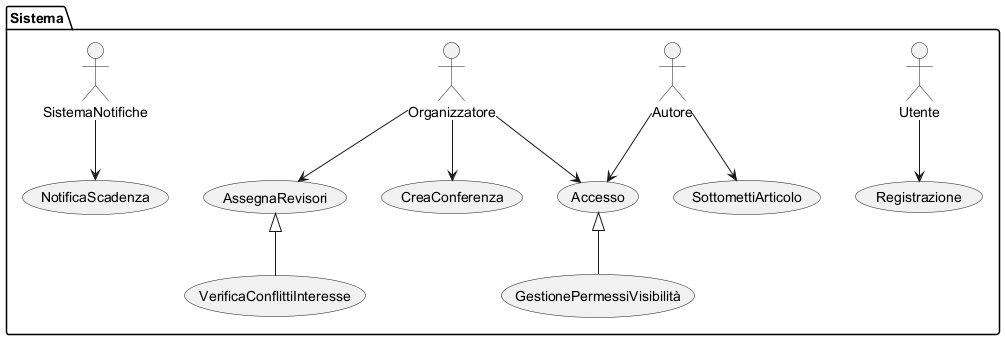
\includegraphics[width=\linewidth]{./VisualParadigm/diagramma_uso.png}
  \caption{Diagramma dei casi d'uso}
  \label{fig:diagramma_uso}
\end{figure}

%%% Local Variables:
%%% mode: LaTeX
%%% TeX-master: "main"
%%% End:

\subsection{Scenari}
\label{sec:scenari}
\begin{tabular}{|p{3cm}|p{7cm}|}
\hline 
\rowcolor{Orchid}
Caso d'uso & Registrazione \\
\hline
Attore Primario & Utente\\
\hline
Attore Secondario & \\
\hline
Descrizione & Permette la registrazione di un utente\\
\hline
  Sequenza Eventi &
                    \begin{enumerate}
                    \item Il caso d'uso inizia quando l'Utente inserisce Nome,Congome, Affiliazione, Email e Password
                    \item Il sistema verifica che l'email non sia utilizzata anche per altri
                    \item Se il controllo è positivo e non si è verifcato alcun errrore
                      \begin{enumerate}
                      \item il sistema informa all'utente la buona uscita dell'operazione e gli assegnerà un ID univoco
                      \end{enumerate}
                    \end{enumerate}\\
\hline
Post-Condizioni: & Il cliente è registrato nel sistema \\
\hline
Sequenza degli eventi alternativa & Al punto 3 il cliente immette una Email non compatibile o che sia già utilizzata restituendo un messaggio di errore\\
\hline
\end{tabular}

\begin{tabular}{|p{3cm}|p{7cm}|}
\hline 
\rowcolor{Orchid}
Caso d'uso & Accesso \\
\hline
Attore Primario & Utente\\
\hline
Attore Secondario & \\
\hline
Descrizione & Permette l'accesso ad un utente al suo account\\
\hline
Pre-Condizioni& L'utente sia già registrato\\
\hline
  Sequenza Eventi&
                   \begin{enumerate}
                   \item Il caso d'uso inizia quando l'Utente inserisce Email E Password
                   \item Il sistema verifica che l'email e  passoword coincidono con l'utente già registrato
                   \item Se il controllo è positivo e non si è verifcato alcun errrore
                     \begin{enumerate}
                     \item il sistema informa all'utente la buona uscita dell'operazione
                     \end{enumerate}
                   \end{enumerate}\\
\hline
Post-Condizioni: &il cliente ha l'accesso al suo account \\
\hline
Sequenza degli eventi alternativa & Al punto 3 il cliente immette una Email collegato ad alcun account  oppure che l'email e passoword non coincidono restituendo un messaggio di errore\\
\hline
\end{tabular}

\begin{tabular}{|p{3cm}|p{7cm}|}
\hline 
\rowcolor{Orchid}
Caso d'uso & Crea Conferenza \\
\hline
Attore Primario & Organizzatore\\
\hline
Attore Secondario & Sistema Di notifica\\
\hline
Descrizione & L'organizzatore crea una conferenza \\
\hline
  Sequenza Eventi &
                    \begin{enumerate}
                    \item L'organizzatore crea una Conferenza inserendo il Titolo, una Descrizione dell'evento e una singola data di scadenza per le sottomissioni
                    \item Il sistema verifica che la data non sia passata o non sia valida
                    \item Se il controllo è positivo e non si è verifcato alcun errrore
                      \begin{enumerate}
                      \item il sistema informa all'utente la buona uscita dell'operazione
                      \item Il sistema permette il monitoraggio dei vari articoli sottomessi per la conferenza
                      \end{enumerate}
                    \end{enumerate}\\
\hline
Post Condizioni: & L'organizzatore crea una conferenza a cui i vari autori possono sottomettere degli articoli \\
\hline
Sequenza degli eventi alternativa & Nel caso in cui la data di scadenza inserita non sia valida o che sia già passata invia un messaggio di errore \\
\hline
\end{tabular}

\begin{tabular}{|p{3cm}|p{7cm}|}
\hline 
\rowcolor{Orchid}
Caso d'uso & SottomettiArticolo \\
\hline
Attore Primario & Autore\\
\hline
Descrizione & L'autore sottomette un articolo per una determinata conferenza\\
\hline
Pre-Condizioni& Esiste la conferenza\\
\hline
  Sequenza Eventi &
                    \begin{enumerate}
                    \item L'autore inserisce un articolo composto da un Titolo,Abstract e dai Co-Autori
                    \item Il sistema inserisce l'articolo e verifica che l'autore e i co-autori siano registrati al sistema
                    \item Se il controllo è positivo e non si è verifcato alcun errrore
                      \begin{enumerate}
                      \item Il sistema informa all'utente la buona uscita dell'operazione
                      \item Il sistema inserisce l'articolo e permette agli autori di poter visualizzare lo stato dell'articolo
                      \end{enumerate}
                    \end{enumerate} \\
\hline
Post-Condizioni: &L'articolo è inserito e possibile per la verica degli articoli da parte dei Revisori\\
\hline
Sequenza degli eventi alternativa & Il sistema nel caso in cui i co-autori non sono stati registrati non procede con l'inserimento dell'articolo e restituisce un messaggio di errore\\
\hline
\end{tabular}

\begin{tabular}{|p{3cm}|p{7cm}|}
\hline 
\rowcolor{Orchid}
Caso d'uso & AssegnaRevisori \\
\hline
Attore Primario & Organizzatore\\
\hline
Attore Secondario & Sistema di notifica\\
\hline
Descrizione &L'organizzatore  assegna ad ogni articolo dei revisori per la revisione dell'articolo\\
\hline
Pre-Condizioni& L'Autore ha sottomesso l'articolo\\
\hline
  Sequenza Eventi&
                   \begin{enumerate}
                   \item Il caso d'uso inizia allo scadere della data di revisione
                   \item L'organizzatore assegna ad ogni articolo sottomesso tre revisori
                   \item L'assegnazione può essere tramite ID oppure scegliendoli dalla lista di quelli registrati
                   \end{enumerate}\\
\hline
Post-Condizioni: &L'articolo passa da uno stato di "sottomesso" a quello di "revisione" \\
\hline
Sequenza degli eventi alternativa & \\
\hline
\end{tabular}
  

\begin{tabular}{|p{3cm}|p{7cm}|}
\hline 
\rowcolor{Orchid}
Caso d'uso & NotificaScadenza \\
\hline
Attore Primario & Sistema di Notifica\\
\hline
Attore Secondario & Autore\\
\hline
Descrizione & Permette la notifica automatica via email per le principali scadenze\\
\hline
Pre-Condizioni& L'utente sia già registrato\\
\hline
  Sequenza Eventi&
                   \begin{enumerate}
                   \item Il caso d'uso inizia quando la scadenza è imminente
                   \item Il sistema invia delle notifiche agli autori per le scadenze delle varie conferenze
                   \item Tramite Email vengono notificati gli autori
                   \end{enumerate}\\
\hline
Post-Condizioni: & \\
\hline
Sequenza degli eventi alternativa & \\
\hline
\end{tabular}

%%% Local Variables:
%%% mode: LaTeX
%%% TeX-master: "main"
%%% End:

%%% Local Variables:
%%% mode: LaTeX
%%% TeX-master: "main"
%%% End:

\section{Diagramma delle Classi}
\subsection{Responsabilita}
\label{sec:responsabilita}
\begin{tabular}{|p{5cm}|p{5cm}|}
\hline 
 \rowcolor{SkyBlue}
RESPONSABILITA & CLASSE\\
\hline
Registrazione & Sistema\\
\hline
Accesso & Sistema\\
\hline
Crea Conferenzza & Organizzatore\\
\hline
Sottometti Articolo & Autore\\
\hline
Assegna Revisori & Organizzatore\\
\hline
Notifica Scadenza & Sistema di Notifiche\\
\hline
Dispositivo di Accesso & Sistema\\
\hline
Gestione Permessi Visibilita & Sistema\\
\hline
Verifica Conflitti di Interesse & Sistema\\
\hline
\end{tabular}

\begin{itemize}
\item Registrazione e Accesso risultano responsabilita della classe Sistema, poiche sta a lui validare i dati e credenziali inserite.\\
\item Crea Conferenzza è responsabilita di Organizzatore, poiche è <<Creator>> di tale classe, andando poi a definire i vari parametri.\\
\item Assegna Revisori è responsabilita di Organizzatore, poiche è <<Creator>> di tale classe, andando ad assegna un revisore per ogni articolo.\\
\item Sottometti Articolo è responsabilita di Autore, poiche è <<Creator>> di tale classe, andando a sottomentere un dato articolo per una coonferenza.\\
\item Notifica Scadenza è responsabilita del Sitema di Notifiche andando ad automitizzando la comunicazione delle scadenze per gli utenti coinvolti.\\
\item Dispositivo di Accesso è responsabilita del Sistema permettere e controllare l'acceso degli Utenti da diversi dispositivi.\\
\item Gestione Permessi Visibilita è responsabilita del Sistema, anadando a gestire permessi.\\
\item Verifica Conflitti di Interesse è responsabilita del Sistema, poiche deve garatire l'assenza di conflitti tra articoli assegnati e rispettivi revisori.\\
\end{itemize}

%%% Local Variables:
%%% mode: LaTeX
%%% TeX-master: "main"
%%% End:

\begin{figure}[!ht]
  \centering
  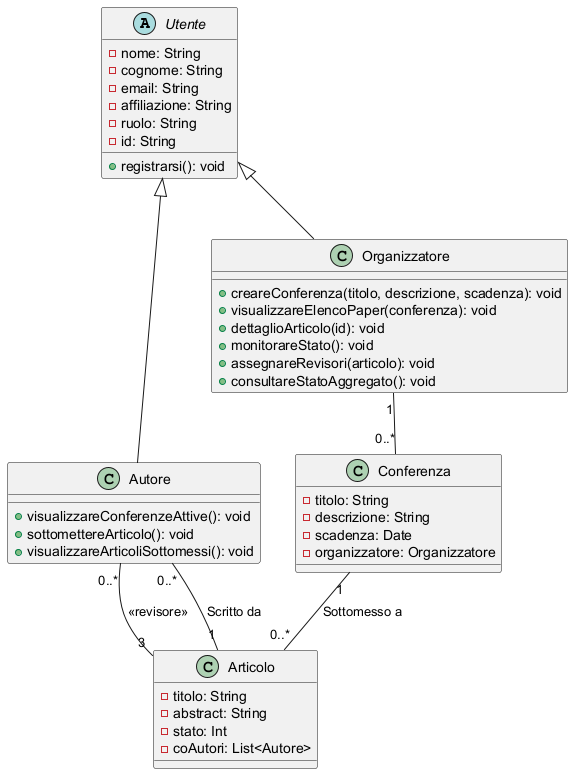
\includegraphics[width=\linewidth]{./VisualParadigm/diagramma_classi.png}
  \caption{Diagramma delle classi}
  \label{fig:diagramma_classi}
\end{figure}
%%% Local Variables:
%%% mode: LaTeX
%%% TeX-master: "main"
%%% End:

\section{Diagramma di Sequenza}
\label{sec:sequenza}
\subsection{Sottomissione di un articolo}
\label{sec:sequenza_sottomissione}
\begin{figure}[ht]
  \centering
  \includegraphics[width=\linewidth]{VisualParadigm/diagramma_sequenza_sottomissione.png}
  \caption{Diagramma di Sequenza per la sottomissione di un articolo}
  \label{fig:sottomissione}
\end{figure}

Dalla creazione del diagramma \ref{fig:sottomissione} si è visto che è
necessario creare un metodo per la verifica delle credenziali,
responsabilità della classe che gestisce la comunicazione con il
database.
%%% Local Variables:
%%% mode: LaTeX
%%% TeX-master: "main"
%%% End:

\subsection{Creazione e gestione conferenza}
\label{sec:sequenza_conferenza}
\begin{figure}[ht]
  \centering
  \includegraphics[width=\linewidth]{VisualParadigm/diagramma_sequenza_conferenza.png}
  \caption{Diagranna di Sequenza per la creazione e gestione di una conferenza}
  \label{fig:conferenza}
\end{figure}

%%% Local Variables:
%%% mode: LaTeX
%%% TeX-master: "main"
%%% End:

\subsection{Assegnazione revisori}
\label{sec:revisori}

\begin{figure}[ht]
  \centering
  \includegraphics[width=\linewidth]{VisualParadigm/diagramma_sequenza_revisori.png}
  \caption{Diagramma di sequenza per l'assegnazione dei revisori}
  \label{fig:revisori}
\end{figure}

%%% Local Variables:
%%% mode: LaTeX
%%% TeX-master: "main"
%%% End:


%%% Local Variables:
%%% mode: LaTeX
%%% TeX-master: "main"
%%% End:

%%% Local Variables:
%%% mode: LaTeX
%%% TeX-master: "main"
%%% End:

\chapter{Piano di Test Funzionale}
\label{sec:piano_di_test_funzionale}
\subsection{Test Registrazione}
\label{sec:test_registrazione}

\begin{sidewaystable}
\begin{tabular}{|p{3.5cm}|p{2cm}|p{2cm}|p{3cm}|p{2cm}|p{2cm}|}
\hline
\rowcolor{SkyBlue}
\multicolumn{6}{l}{\textbf{REGISTRAZIONE}}\\
\hline
\rowcolor{Red}
\textbf{Nome} & \textbf{Cognome} & \textbf{Email} & \textbf{Password} & \textbf{Affiliazione} & \textbf{Ruolo}  \\
\hline
Stringa di caratteri di lunghezza <=30 & Stringa di caratteri di lunghezza <=30 & Stringa con @ in posizione valida e non già registrata & Stringa alfanumerica con 2 caratteri speciali e lunghezza ≤ 40 & Stringa alfanumerica di lunghezza ≤ 50, senza simboli & Autore o Organizzatore \\
\hline
Stringa alfabetica di lunghezza > 30 → [ERROR] & Stringa alfabetica di lunghezza > 30 → [ERROR] & Stringa con @ ma già registrata → [ERROR] & Stringa con meno di 2 caratteri speciali o senza → [ERROR] & Stringa senza @ → [ERROR] & Qualsiasi altro valore → [ERROR] \\
\hline
Stringa con caratteri speciali → [ERROR] & Stringa alfabetica di lunghezza > 30 → [ERROR] & Stringa senza @ → [ERROR] & Stringa con caratteri non alfanumerici validi → [ERROR] & Stringa con caratteri speciali → [ERROR] & Campo vuota → [ERROR]  \\
\hline
Stringa vuota → [ERROR] & Stringa vuota → [ERROR] & Stringa vuota → [ERROR] & Stringa con lunghezza > 40 → [ERROR] & Stringa vuota → [ERROR] &\\
\hline
\end{tabular}
\end{sidewaystable}

\begin{itemize}
\item Il numero di test da fare senza vincoli particolari è: 1 x 1 x 1 x 1 x 2 = 6
\item Con i vincoli [ERROR], il numero di test da fare per testare singolarmente i vincoli è 3 per Nome, 3 per Cognome, 3 per Email, 3 per Affiliazione, 2 per Ruolo = 14 
\item Il numero di test risultante è: (1 × 1) + 14 = 15.
\end{itemize}

\begin{sidewaystable}
\begin{tabular}{|p{3cm}|p{2cm}|p{2cm}|p{2cm}|p{4cm}|p{2cm}|p{2cm}|}
\hline
\rowcolor{SkyBlue}
\multicolumn{7}{l}{\textbf{Test Suite: Registrazione 1}} \\
\hline
\rowcolor{Red}
\textbf{Test Case ID} & \textbf{Descrizione} & \textbf{Classi di Equivalenza} & \textbf{Pre-condizioni} & \textbf{Input} & \textbf{Output Atteso} & \textbf{Post-condizioni} \\
\hline
1 & Tutti input validi & Nome valido, Cognome valido, Email valida non registrata, Password valida, Affiliazione valida, Ruolo valido & Nessuna & \texttt{\{Nome: "Mario", Cognome: "Calcagno", Email: "mario@email.com", Password: "Mario!@1234", Affiliazione: "Politecnico", Ruolo: "attore"\}} & Utente registrato con successo & Si riceve email di conferma \\
\hline
2 & Nome $>$ 30 caratteri & Nome troppo lungo, altri campi validi & Nessuna & \texttt{\{Nome: "Giuseppemeravigliosissimodavvero", Cognome: "Buglione", Email: "giuseppe@email.com", Password: "Pass@12!!", Affiliazione: "Uniba", Ruolo: "organizzatore"\}} & Errore: nome troppo lungo & \\
\hline
3 & Cognome con simboli & Cognome con caratteri speciali [ERROR], altri campi validi & Nessuna & \texttt{\{Nome: "Francesco", Cognome: "Calc@lli", Email: "francesco@email.com", Password: "Francesco]]22", Affiliazione: "Uniba", Ruolo: "autore"\}} & Errore: formato cognome non valido & \\
\hline
4 & Email già registrata & Email duplicata [ERROR], altri campi validi & Email già usata da altro utente & \texttt{\{Nome: "Mario", Cognome: "Calcagno", Email: "mario@email.com", Password: "M@rio123!!", Affiliazione: "Politecnico", Ruolo: "autore"\}} & Errore: email già in uso & \\
\hline
\end{tabular}
\end{sidewaystable}

\begin{sidewaystable}
\begin{tabular}{|p{3cm}|p{2cm}|p{2cm}|p{2cm}|p{4cm}|p{2cm}|p{2cm}|}
\hline
\rowcolor{SkyBlue}
\multicolumn{7}{l}{\textbf{Test Suite: Registrazione 2}}\\
\hline
\rowcolor{Red}
\textbf{Test Case ID} & \textbf{Descrizione} & \textbf{Classi di Equivalenza} & \textbf{Pre-condizioni} & \textbf{Input} & \textbf{Output Atteso} & \textbf{Post-condizioni} \\
\hline
5 & Email senza “@” & Email malformata [ERROR], altri campi validi & Nessuna & \texttt{\{Nome: "Giuseppe", Cognome: "Buglione", Email: "giuseppeemail.com", Password: "Gius!@1234", Affiliazione: "Uniba", Ruolo: "organizzatore"\}} & Errore: formato email errato & \\
\hline
6 & Password troppo corta & Password con meno di 2 caratteri speciali [ERROR], altri campi validi & Nessuna & \texttt{\{Nome: "Francesco", Cognome: "Calculli", Email: "francesco.new@email.com", Password: "Francesco123", Affiliazione: "Uniba", Ruolo: "autore"\}} & Errore: password non sicura & \\
\hline
7 & Affiliazione con simboli & Affiliazione con caratteri speciali [ERROR], altri campi validi & Nessuna & \texttt{\{Nome: "Mario", Cognome: "Calcagno", Email: "mario2@email.com", Password: "Mario!!44", Affiliazione: "Politec@nico", Ruolo: "organizzatore"\}} & Errore: formato affiliazione errato & \\
\hline
8 & Ruolo non valido & Ruolo non previsto [ERROR], altri campi validi & Nessuna & \texttt{\{Nome: "Giuseppe", Cognome: "Buglione", Email: "giuseppe2@email.com", Password: "Pass@@12", Affiliazione: "Uniba", Ruolo: "manager"\}} & Errore: ruolo non valido & \\
\hline
\end{tabular}
\end{sidewaystable}

%%% Local Variables:
%%% mode: LaTeX
%%% TeX-master: "main"
%%% End:

\subsection{Test Accesso}
\label{sec:test_accesso}

\begin{tabular}{|p{6cm}|p{6cm}|}
\hline
\rowcolor{SkyBlue}
\textbf{ACCESSO	} & \\
\hline
\rowcolor{Red}
\textbf{Email} & \textbf{Password} \\ 
\hline
Stringa valida contenente “@” e registrata nel sistema & Stringa corretta, associata all’email inserita  \\
\hline
Stringa valida ma non registrata → [ERROR] &   Stringa errata → [ERROR] \\
\hline
Stringa senza “@” o in formato errato → [ERROR] &  Stringa vuota o non conforme → [ERROR] \\
\hline
\end{tabular}

\begin{itemize}
\item Il numero di test da fare senza vincoli particolari è: 1 × 1 = 1.
\item Con i vincoli [ERROR], il numero di test da fare per testare singolarmente i vincoli è 4 (2 per Email, 2 per Password). 
\item Il numero di test risultante è: (1 × 1) + 4 = 5.
\end{itemize}

\begin{sidewaystable}
\begin{tabular}{|p{2cm}|p{2cm}|p{2cm}|p{2cm}|p{5cm}|p{2cm}|p{2cm}|}
\hline
\rowcolor{SkyBlue}
\multicolumn{7}{l}{\textbf{Test Suite: Accesso}}\\
\hline
\rowcolor{Red}
\textbf{Test Case ID} & \textbf{Descrizione} & \textbf{Classi di Equivalenza} & \textbf{Pre-condizioni} & \textbf{Input} & \textbf{Output Atteso} & \textbf{Post-condizioni} \\
\hline
1 & Accesso con credenziali valide & Email valida e registrata, Password corretta & Email e password già registrate & \texttt{\{Email: "mario@email.com", Password: "Mario!@1234"\}} & Accesso consentito & Sessione utente avviata \\
\hline
2 & Email non registrata & Email valida ma non presente [ERROR] & Nessuna & \texttt{\{Email: "nonregistrata@email.com", Password: "Qualcosa!@1"\}} & Errore: utente non trovato & \\
\hline
3 & Email senza “@” & Email malformata [ERROR] & Nessuna & \texttt{\{Email: "giuseppemail.com", Password: "Pass@12!!"\}} & Errore: formato email errato & \\
\hline
4 & Password errata & Email registrata, password sbagliata [ERROR] & Email registrata nel sistema & \texttt{\{Email: "buglione@email.com", Password: "passwordSbagliata!!"\}} & Errore: credenziali non valide & \\
\hline
5 & Password vuota & Email valida e registrata, Password vuota [ERROR] & Email registrata nel sistema & \texttt{\{Email: "calculli@email.com", Password: ""\}} & Errore: password mancante & \\
\hline
6 & Email e password errati & Email malformata + password errata [ERROR] & Nessuna & \texttt{\{Email: "francescoemail.com", Password: "123"\}} & Errore: formato email errato & \\
\hline
\end{tabular}
\end{sidewaystable}

%%% Local Variables:
%%% mode: LaTeX
%%% TeX-master: "main"
%%% End:

\subsection{Test Creazione Conferenza}
\label{sec:test_creaszione_conferenzza}

\begin{tabular}{|p{3.5cm}|p{2cm}|p{2cm}|p{3cm}|}
\hline
\rowcolor{SkyBlue}
\textbf{CREAZIONE CONFERENZA} & & &\\
\hline
\rowcolor{Red}
\textbf{Organizzatore} & \textbf{Titolo} & \textbf{Descrizione} & \textbf{Scadenza}  \\
\hline
 Utente con ruolo "organizzatore" & Stringa ≤ 70 caratteri alfanumerici e speciali &  Stringa ≤ 300 caratteri & Data futura (valida) \\
Utente con ruolo non valido → [ERROR] &  Stringa > 70 caratteri → [ERROR] & Stringa > 300 caratteri → [ERROR] & Data passata → [ERROR] \\
Utente con ruolo mancante → [ERROR] & Stringa vuota → [ERROR] &  & Data odierna → [ERROR] \\
& & & Formato errato → [ERROR] \\
\hline
\end{tabular}

\begin{itemize}
\item Il numero di test da fare senza vincoli particolari è: 1×1×1×1=1.
\item Con i vincoli [ERROR], il numero di test da fare per testare singolarmente i vincoli è : 1 (Per Org. non valido) + 2 (Per Titolo[troppo lungo, vuoto]) +1 (Per Descr. troppo lunga) + 1 (Per Scadenza errata) = 5
\item Il numero di test risultante è: 1 + 5 = 6.
\end{itemize}

\begin{sidewaystable}
\begin{tabular}{|p{2cm}|p{2cm}|p{2cm}|p{2cm}|p{5cm}|p{2cm}|p{2cm}|}
\hline
\rowcolor{SkyBlue}
\multicolumn{7}{l}{\textbf{Test Suite: Ceazione Conferenza}}\\
\hline
\rowcolor{Red}
\textbf{Test Case ID} & \textbf{Descrizione} & \textbf{Classi di Equivalenza} & \textbf{Pre-condizioni} & \textbf{Input} & \textbf{Output Atteso} & \textbf{Post-condizioni} \\
\hline
1 & Conferenza valida & Organizzatore valido, Titolo ≤70, Descrizione ≤300, Scadenza valida & Utente loggato come organizzatore & \texttt{\{Organizzatore: "Mario", Titolo: "Conf AI", Descrizione: "Evento su AI", Scadenza: "2025-12-01"\}} & Conferenza creata con successo & Conferenza salvata \\
\hline
2 & Utente non organizzatore & Organizzatore non valido [ERROR] & Utente loggato & \texttt{\{Organizzatore: "Giuseppe", Ruolo: "attore", ...\}} & Errore: permesso negato & \\
\hline
3 & Titolo troppo lungo & Titolo > 70 caratteri [ERROR] & Organizzatore valido & \texttt{\{Titolo: "AAAAAAAAAA... (80 caratteri)", ...\}} & Errore: titolo troppo lungo & \\
\hline
4 & Titolo vuoto & Titolo vuoto [ERROR] & Organizzatore valido & \texttt{\{Titolo: "", ...\}} & Errore: titolo mancante & \\
\hline
5 & Descrizione troppo lunga & Descrizione > 300 caratteri [ERROR] & Organizzatore valido & \texttt{\{Descrizione: "A...A" (301 caratteri), ...\}} & Errore: descrizione troppo lunga & \\
\hline
6 & Scadenza non valida & Scadenza passata o malformata [ERROR] & Organizzatore valido & \texttt{\{Scadenza: "2022-01-01"\}} & Errore: scadenza non valida & \\
\hline
\end{tabular}
\end{sidewaystable}

%%% Local Variables:
%%% mode: LaTeX
%%% TeX-master: "main"
%%% End:

\subsection{Test Sottomissione di un articolo}
\label{sec:test_sottomissione}
\begin{tabular}{|p{4cm}|p{4cm}|p{4cm}|}
  \hline
  \rowcolor{SkyBlue}
  \textbf{Sottomisione di un articolo} & & \\
  \hline
    \rowcolor{Red}
  \textbf{Titolo} & \textbf{Abstract} & \textbf{Co-Autori} \\
  \hline
  Stringa di caratteri di lunghezza \(\leq 150\)  & Stringa di caratteri di lunghezza \(\leq 250\) & Lista dei co-autori \\
  \hline
  Stringa di caratteri di lunghezza \(> 150 \rightarrow\) [ERROR] & Stringa di caratteri di lunchezza \(> 250 \rightarrow\) [ERROR]& Numero di co-autori \(> 3 \rightarrow\) [ERROR]\\
  \hline
   & & Non tutti i co-autori sono già registrati nel sistema\\
  \hline
\end{tabular}
\begin{itemize}
\item Numero di test fatti senza particolari vincoli risulta: \(2\cdot2\cdot3 = 12\)
\end{itemize}

\begin{sidewaystable}
  \small
  \centering
  \begin{tabular}{|p{2cm}|p{3cm}|p{3cm}|p{3cm}|p{3cm}|p{3cm}|p{2.5cm}|}
    \hline
    \rowcolor{SkyBlue}
    \multicolumn{7}{l}{\textbf{Test Suite: Sottomissione di un articolo}}\\
    \hline
        \rowcolor{Red}
    \textbf{Test Case ID} & \textbf{Descrizione} & \textbf{Classi di equivalenza} & \textbf{Pre\hyp{}condizioni} & \textbf{Input} & \textbf{Output attesi} &\textbf{Post\hyp{}condizioni attese }\\
    \hline
    1 & Tutti gli input validi & titolo valido abstract valido co-autori validi & I co\hyp{}autori sono già presenti nel sistema & \texttt{Titolo: 'L'empatia nei topi', Abstract:'Come l'empatia cambia il comportamento dei topi', co-autori: ['3304', '43044', '54423']}& Articolo Sottomesso & Lo stato dell'articolo viene impostato a sottomesso \\
    \hline
    2 & Titolo stringa \(>150\) caratteri & Stringa di caratteri di lunghezza \(> 150 \rightarrow\) [ERROR]  & & \texttt{Titolo: '00000000000...', Abstract:'Come l'empatia cambia il comportamento dei topi', co-autori: ['3304', '43044', '54423']} & Titolo troppo lungo & \\
    \hline
    3 & abstract stringa \(> 250\) & Stringa di caratteri di lunchezza \(> 250 \rightarrow\) [ERROR] & &  \texttt{Titolo: 'L'empatia nei topi', Abstract:'0000...', co-autori: ['3304', '43044', '54423']} & Abstract troppo lungo & \\
    \hline
    4 & co\hyp{}autori \(> 3\) & Numero di co-autori \(> 3 \rightarrow\) [ERROR] & &\texttt{Titolo: 'L'empatia nei topi', Abstract:'Come l'empatia cambia il comportamento dei topi', co-autori: ['3304', '43044', '54423', '64132']} & Troppi co\hyp{}autori & \\
    \hline
    5 & co\hyp{}autori non registrati & Non tutti i co-autori sono già registrati nel sistema \(rightarrow\) [ERROR]  & &\texttt{Titolo: 'L'empatia nei topi', Abstract:'Come l'empatia cambia il comportamento dei topi', co-autori: ['3304', '43044', '54423']} & co\hyp{}autore non trovato & \\
    \hline
  \end{tabular}
\end{sidewaystable}

%%% Local Variables:
%%% mode: LaTeX
%%% TeX-master: "main"
%%% End:

\subsection{Test Assegna Revisori}
\label{sec:test_assegna_revisori}

\begin{tabular}{|p{3.5cm}|p{3cm}|p{3cm}|p{3cm}|}
\hline
\rowcolor{SkyBlue}
\multicolumn{4}{l}{\textbf{ASSEGNA REVISORE}}\\
\hline
\rowcolor{Red}
\textbf{Nome Articolo} & \textbf{ID Revisore 1} & \textbf{ID Revisore 2} & \textbf{I Revisore 3}  \\
\hline
Stringa di caratteri non vuota di un articolo già esistente di lunghezza <=100 & ID di Autori,distinti, che non sono Autori e Co-autori dell'articolo & ID di Autori,distinti, che non sono Autori e Co-autori dell'articolo & ID di Autori,distinti, che non sono Autori e Co-autori dell'articolo \\
\hline
Nome dell'articolo non esistente→ [ERROR]& ID Autori che hanno scritto l'articolo →[ERROR] & ID Autori che hanno scritto l'articolo →[ERROR] & ID Autori che hanno scritto l'articolo →[ERROR]\\
\hline
Stringa con caratteri speciali→[ERROR]&   ID Autore duplicato→[ERROR] & ID Autore duplicato→[ERROR] & ID Autore duplicato→[ERROR] \\
\hline
Stringa vuota → [ERROR]&ID Autore nullo→[ERROR]& ID Autore nullo→[ERROR & ID Autore nullo→[ERROR \\
\hline
Stringa di lunghezza>100 →[ERROR]&  ID Organizzatore→[ERROR] &  ID Organizzatore→[ERROR] &  ID Organizzatore→[ERROR] \\
\hline
& ID Autore non esistente→[ERROR] & ID Autore non esistente→[ERROR] & ID Autore non esistente→[ERROR] \\
\hline
\end{tabular}

\begin{itemize}
\item Numero di test fatti senza particolari vincoli risulta:1
\item Numero di test con vincoli risulta: 4 Per Nome Articolo, 5 per IDRevisore = 9 
\item  Il numero di test risultante è: 1+ 9 = 10
\end{itemize}
 
\begin{sidewaystable}
\begin{tabular}{|p{3cm}|p{2cm}|p{2cm}|p{2cm}|p{4cm}|p{2cm}|p{2cm}|}
\hline
\rowcolor{SkyBlue}
  \multicolumn{7}{l}{\textbf{Test Suite: Assegna Revisore 2}}\\
\hline
\rowcolor{Red}
\textbf{Test Case ID} & \textbf{Descrizione} & \textbf{Classi di Equivalenza} & \textbf{Pre-condizioni} & \textbf{Input} & \textbf{Output Atteso} & \textbf{Post-condizioni} \\
\hline
1& Tutti gli input validi &NomeArticolo Valido,IDRevisore1 Valido, ID Revisore2 Valido, IDRevisore3 Valido&NomeArticolo Presente, IDRevisore1/IDRevisore2/IDRevisore3 Autori& NomeArticolo: Studio AI , IDRevisore1: 10,IDRevisore2:11, IDRevisore3:12&Articolo in revisione& Stato di Articolo cambiato da "Sottomesso" a "In Revisione"\\
\hline
2& NomeArticolo non esistente&NomeArticolo non esistente, Revisori validi& IDRevisore1/IDRevisore2/IDRevisore3 Autori& NomeArticolo: Computer Quantistici, IDRevisore1: 10,IDRevisore2:11, IDRevisore3:12&Errore: Nome Articolo Non Esistente&\\
\hline
3& NomeArticolo con con caratteri speciali& NomeArticolo con caratteri speciali, Revisori Validi & IDRevisore1/IDRevisore2/IDRevisore3 Autori& NomeArticolo: ***, IDRevisore1: 10,IDRevisore2:11, IDRevisore3:12&Errore: Nome Articolo Presenta dei caratteri speciali &\\
\hline
4&NomeArticolo vuoto & NomeArticolo:Stringa Vuota, Revisori Validi & IDRevisore1/IDRevisore2/IDRevisore3 Autori& NomeArticolo:None , IDRevisore1: 10,IDRevisore2:11, IDRevisore3:12&Errore:Nome Artivolo Vuoto&\\
\hline
5&Nome Articolo stringa>100 &Nome Articolo >100 caratteri , Revisori Validi & IDRevisore1/IDRevisore2/IDRevisore3 Autori&NomeArticolo:Stuuuuuuuuuuuuuuuudio AI,  IDRevisore1: 10,IDRevisore2:11, IDRevisore3:12&Errore: Nome Articolo Troppo lungo&\\
\hline 
\end{tabular}
\end{sidewaystable}

\begin{sidewaystable}
\begin{tabular}{|p{3cm}|p{2cm}|p{2cm}|p{2cm}|p{4cm}|p{2cm}|p{2cm}|}
\hline
\rowcolor{SkyBlue}
\multicolumn{7}{l}{\textbf{Test Suite: Assegna Revisore 1}}\\
\hline
\rowcolor{Red}
\textbf{Test Case ID} & \textbf{Descrizione} & \textbf{Classi di Equivalenza} & \textbf{Pre-condizioni} & \textbf{Input} & \textbf{Output Atteso} & \textbf{Post-condizioni} \\
\hline
6&IDRevisore Scrittori Articolo& Nome Articolo Valido, IDRevisore1 autore articolo, gli altri revisori sono validi&NomeArticolo Presente, IDRevisore1/IDRevisore2/IDRevisore3 Autori&NomeArticolo: Studio AI , IDRevisore1: 1,IDRevisore2:11, IDRevisore3:12&Errore: Almeno un revisore è Autore dell'articolo &\\
\hline
7&IDRevisore duplicato& NomeArticolo Valido, IDRevisore1=IDRevisore2,IDRevisore3 valido &NomeArticolo Presente, IDRevisore1/IDRevisore2/IDRevisore3 Autori&NomeArticolo: Studio AI , IDRevisore1: 11,IDRevisore2:11, IDRevisore3:12&Errore: Almeno un revisore è duplicato &\\
\hline
8&IDRevisore Nullo& Nome Articolo Valido, IDRevisore1 nullo, gli altri revisori validi&NomeArticolo Presente,IDRevisore2/IDRevisore3 Autore& NomeArticolo: Studio AI , IDRevisore1: None,IDRevisore2:11, IDRevisore3:12& Errore: Almeno un revisore è nullo&\\
\hline
9&ID Revisore è un organizzatore&Nome Articolo Valido, IDRevisore1 organizzatore, gli altri revisori sono validi & Nome Articolo Presente, IDRevisore1 Organizzatore, IDRevisore2/IDRevisore3 Autori& NomeArticolo: Studio AI , IDRevisore1: 32,IDRevisore2:11, IDRevisore3:12&Errore: Almeno un Revisore è Organizzatore&\\
\hline
10&ID Rebisore non esistente&Nome Articolo Valido, IDRevisore non esistente, gli altri revisori sono validi & Nome articolo Presente, IDRevisore2/IDRevisore3 Autori&NomeArticolo: Studio AI , IDRevisore1: 312,IDRevisore2:11, IDRevisore3:12&Errore: Almeno un revisore non esiste&\\
\hline 
\end{tabular}
\end{sidewaystable}

%%% Local Variables:
%%% mode: LaTeX
%%% TeX-master: "main"
%%% End:


%%% Local Variables:
%%% mode: LaTeX
%%% TeX-master: "main"
%%% End:

\chapter{Progettazione}
\label{sec:progettazione}
\section{Diagramma delle Classi}
\label{sec:diagramma_delle_classi}
\begin{figure}[ht]
  \centering
  \includegraphics[width=\linewidth]{VisualParadigm/diagramma_prg_classi.png}
  \caption{Diagramma delle classi}
  \label{fig:prg_diagramma_classi}
\end{figure}

%%% Local Variables:
%%% mode: LaTeX
%%% TeX-master: "main"
%%% End:

\subsection{Traduzione classi ed associazioni}
\label{sec:prg_traduzione}

In tale \textbf{sezione} si va esplicitare il processo che dal modello concettuale ci porta al modello di progettazione, basato sull'architettura \textbf{BCED} (\textbf{Boundary}, \textbf{Controller}, \textbf{Entity}, \textbf{Database}).
Dove le scelte di progettazione sono state influenzzate da:
\begin{itemize}
\item Vincoli e le funzionalità espresse nei requisiti \ref{sec:analisi_nomi_verbi}
\item Rispettare i vicoli del modello \textbf{BCED}
\end{itemize}

\paragraph{Classi Entity}
\begin{description}
\item [User] Generalizzazione del concetto di utente, classe astratta, poiche nel sistema un user può essere solo o un \textbf{author} o un \textbf{organizer}. Caratterizatto dagli segueni attributi:
\begin{itemize}
\item ID: Che va a indetificare in maniera \textbf{univoca} un user
\item Name: nome dell'user
\item Lastname: cognome dell'user
\item Email: elemento identificativo per l'accesso al database per l'user
\item Password:  elemento identificativo per l'accesso al database per l'user 
\item Affiliazzione: organnizazione di appartenenza dell'user
\end{itemize}
\item [Author] Estende la classe \textbf{User}, ereditando tutti gli attributi e metodi. Caratterizzato dall'attributo:
\begin{itemize}
\item Final-Role: indica il ruolo dell'user (in questo caso \textbf{Autore})
\end{itemize}
\item [Organizer] Estende la classe \textbf{User}, ereditando tutti gli attributi e metodi. Caratterizzato dall'attributo:
\begin{itemize}
\item Final-Role: indica il ruolo dell'user (in questo caso \textbf{Organizzatore}) 
\end{itemize}
\item [Conference] rappresenta una conferenza creata da un \textbf{organizer}, caratterizzata dagli seguenti attributi:
\begin{itemize}
\item Titolo: Il nome della conferenzza
\item Descrizione: descrizione dell'argomento su cui è incetratta la conferenzza
\item Scadenza: data di scadenzza per la consegna degli articoli
\item Articoli: lista di riferimenti agli articoli sottomessi
\end{itemize}
\item [Article] rappresenta un articolo sottomesso, caratterizzato dagli seguenti attributi:
\begin{itemize}
 \item Titolo: Titolo dell'articolo
\item Abstract: Contenuto dell'articolo
\item Co-Autori: lista di riferimenti degli auto che hanno partecipato alla creazione dell'articolo
\end{itemize}
\end{description}

\paragraph{Associazioni}
\begin{description}
\item [Organizer->Conference] associazione di tipo: \textbf{1->* [uno a molti]} indica che uno stesso organizzatore può creare più conferenze
\item [Conference->Article] associazione di tipo: \textbf{1->* [uno a molti]} dove una confderenza può avere da uno a più articoli
\item [Author->Article] associazione di tipo: \textbf{*->* [molti a molti]} dove un articolo può essere scrito da uno o più autori mentre quest'ultimi possono scrivere più articoli.
\item [Article->Author] associazione di tipo: \textbf{*->3 [molti a molti]} con cui ad un aticolo si possono assegnare un messimo di 3 revisore attraverso ReviewDAO e ReviewController in particolar modo con:
\begin{itemize}
 \item assignReviewer(articleId, reviewerId)
\item getReviewersForArticle(articleId)
\end{itemize}
\end{description}

\paragraph{Controller}
\begin{description}
\item[TODO]
\end{description}

\paragraph{Data Access Layer}
\begin{description}
\item[TODO]
\end{description}

%%% Local Variables:
%%% mode: LaTeX
%%% TeX-master: "main"
%%% End:

\subsection{Pattern BCED}
\label{sec:pattern_bced}
\subsubsection{Package Boundary}
\label{sec:package_boundary}

Nel Package Boundary vi sono tutti gli oggetti responsabili della costruzione della GUI e della logica di presentazione. A questo livello tutte le classi corrispondono a delle interfacce. 

\paragraph{AssignReviewsView}
Permette la visualizzazione di tutti gli articoli sottomessi all'organizzatore per poter essere poi essere messi in revisione.
\begin{itemize}
\item showPendingReviewers(): Effettua la visualizzazione degli atricoli inoltrati dagli Autori per essere revisionati.\\
\item assingReviewers(): L'organizzatore tramite questa funzione assegna per ogni articolo tre revisori. Nel caso in cui si verificasse un errore viene visualizzato il messaggio di errore da mostrare, altrimenti vengono correttamente assegnati i revisori all'articolo.\\
\end{itemize}


\paragraph{CreateConferenceForm}
L'organizzatore tramite questa classe permette la creazione delle conferenze.\\
\begin{itemize}
\item displayForm(): si occupa della formattazione del form.\\
\item createConference(): L'organizzatore inserisce i dati per la creazione della conferenza, inserendo il titolo, la descrizione, la data di scadenza. Nel caso in cui si verificasse un errore viene visualizzato attraverso un messaggio di errore.
\end{itemize}

\paragraph{LoginView}
Permette la visualizzazione all'utente i form per la registrazione ed l'accesso\\
\begin{itemize}
\item showLoginForm(): Mostra il form per l'accesso dell'utente all'applicazione\\
\item showRegistrationForm(): Mostra il form per la registrazione dell'utente all'applicazione\\
\item handleLogin(): Gestisce l'accesso dell'utente all'applicazione, visualizzando il messaggio di errore quando esso viene riscontrato\\
\item handleRegistration(): Gestisce la registrazione dell'utente all'applicazione, visualizzando quando il messaggio di errore quando viene riscontrato\\
\end{itemize}

\paragraph{RegistrationForm}
Permette la compilazione e l'inoltro del form per la registrazione, permettendo la creazione di un nuovo utente\\
\begin{itemize}
\item displayForm(): Permette la visualizzazione del form per effettuare la registrazione\\
\item submitRegistration(): Inoltra i dati per la registrazione al database, effettuando la verifica dell'inserimento corretto dei dati e nel caso in cui sia già registrato un utente\\
\end{itemize}

\paragraph{LoginForm}
Permette la compilazione e l'intoltro del form per l'accesso, permettendo tramite l'inserimento dell'email e della password dell'account, di accede alla propria dashboard
\begin{itemize}
\item displayForm(): Permette la visualizzazione del form per la compilazione del login
\item submitLogin(): Inoltra i dati inseriti per l'accesso, verificcando attraverso il database l'esistenza dell'utente
\end{itemize}


\paragraph{OrganizerDashboard}
Tramite questa dashboard, vengono visualizzati tutte le conferenze con la possibilità di analizzare anche gli articoli che sono stati sottomessi\\
\begin{itemize}
\item showConferenceList(): Permette la visualizzazione tramite una lista delle conferenze\\
\item viewStats(): Visualizza le statistiche riguardanti le conferenze, tra cui quelle che sono attive. Introduce anche la possibilità di visualizzare gli articoli che sono stati sottomessi per la conferenza determinata\\
\end{itemize}

\paragraph{SubmitArticleForm}
Permette la visualizzazione del form per la sottomissione degli articoli\\
\begin{itemize}
\item displayForm(): Si occupa della visualizzazione del form pe la sottomissione degli articoli\\
\item submitArticle(): Inserendo l'articolo e la conferenza, inoltra l'articolo per la determinata conferenza\\
\end{itemize}

\paragraph{AuthorDashboard}
Tramite questa dashboard, l'autore ha la possibità di visualizzare le conferenze attive e gli articoli sottomessi da lui stesso\\
\begin{itemize}
\item showActiveConference(): Mostra le confereneze attive a cui è possibile sottomettere degli articoli\\
\item showSubmittedArticles(): Mostra gli articoli sottomessi e a quali conferenze sono stati sottomessi\\
\end{itemize}



%%% Local Variables:
%%% mode: LaTeX
%%% TeX-master: "main"
%%% End:

\subsubsection{Package Controller}

\label{sec:package_controller}
\begin{figure}[ht]
  \centering
  \includegraphics[width=\linewidth]{VisualParadigm/diagramma_prg_controller.png}
  \caption{Package Controller}
  \label{fig:Package Controller}
\end{figure}

Il \texttt{package Controller} contiene le classi che si occupano delle
responsabilità, in particolare dei requisiti funzionali (vedere \ref{sec:requisiti_funzionali}).
In particolare abbiamo:
\begin{description}
\item[UserController] Si occupa del login e della registrazione
\item[ConferenceController] Si occupa di creare le conferenze e di richiedere
  i dati relative ad esse tramite le classi DAO
\item[ArticleController] Si occupa della sottomissione degli articoli, di ottenere gli articoli dato un autore e di aggiornare lo stato di un articolo.
\item[ReviewController] Si occupa di assegnare i revisori ad un articolo
\end{description}

%%% Local Variables:
%%% mode: LaTeX
%%% TeX-master: "main"
%%% End:

\subsubsection{Package Entity}
\label{sec:entity}
\begin{figure}[ht] \centering
  \includegraphics[width=\linewidth]{VisualParadigm/diagramma_prg_entity.png}
  \caption{Diagramma delle classi del pacchetto Entity}
  \label{fig:diagramma_entity}
\end{figure}

Il pacchetto Entity contiene le classi di dominio, cioè
le entità trovate durante l'analisi dei nomi e verbi (vedere la
sezione \ref{sec:analisi_nomi_verbi}).

In particolare:
\begin{description}
\item[User] Un utente del sistema
\item[Autore] Un autore, specializza User
\item[Organizzatore] organizza le conferenze, specializza User
\item[Conferenza] una conferenza didattica
\end{description}
%%% Local Variables:
%%% mode: LaTeX
%%% TeX-master: "main"
%%% End:

\subsubsection{Package DTO}

\label{sec:package dto}
\begin{figure}[ht]
  \centering
  \includegraphics[width=\linewidth]{VisualParadigm/diagramma_prg_dto.png}
  \caption{Package DTO}
  \label{fig:Package DTO}
\end{figure}

il \texttt{package DTO} attraverso cui si va a mostrare sulla \texttt{GUI} collezioni di elementi. La cui introduzione nasce dall'esigenza di evirtare un accoppiamento troppo elevato tra package Controller e Entity. Ed è caraterizzato da:
\begin{description}
\item[PossibleReviewDTO] classe DTO per il trasporto delle informazioni di un revisore [autore]
\item[RUserDTO] classe DTO per il trasporto delle informazioni di un utente
\item[ShowActiveConferenceDTO] classe DTO per il trasporto delle informazioni di una conferenzza attiva
\item[ShowArticleDTO] classe DTO per il trasporto delle informazioni di un articolo
\end{description}
%%% Local Variables:
%%% mode: LaTeX
%%% TeX-master: "main"
%%% End:

\subsubsection{Package Database}
\begin{figure}[ht]
  \centering
  \includegraphics[width=\linewidth]{VisualParadigm/diagramma_prg_database.png}
  \caption{Diagramma delle classi del package Database}
  \label{fig:package_database}
\end{figure}

Il \texttt{package Database} contiene le classi che gestiscono la connesione
alla base dati. In particolare si è deciso di utilizzare un approccio basato
su Data Access Object, così da incapsulare la logica di accesso al database
senza che i livelli superiori se debbano occupare.
Le classi qui definite sono:
\begin{description}
\item[DBManager], è la classe che si occupa di creare la connesione al database, tramite protocollo ODBC
\item[UserDAO], è la classe che si occupa di gestire l'accesso alla tabella Utenti nella base di dati
\item[ConferenceDAO], è la classe che si occupa di gestire l'accesso alla tabella Conferenze nella base di dati
\item[ArticleDAO], è la classe che si occupa di gestire l'accesso alla tabella Articoli nella base di dati
\item[ReviewDAO], è la classe che si occupa di gestire i reviewers nella base di dati
\end{description}

\paragraph{DBManager}
La classe DBManager presenta due metodi:
\begin{description}
\item[Costruttore] Costruttore che inizializza la connesione tra il sistema e la base di dati tramite ODBC
\item[getConnection] Getter per la connesione, utilizzato dalle altre classi
  per poter comunicare con la base di dati, senza avere la responsabilità di
  dover gestire la connesione stessa
\end{description}

\paragraph{UserDAO}
La classe UserDAO presenta i seguenti metodi:
\begin{itemize}
\item getUserRoleByID
\item getUserByID
\item isUserPresentByID
\item isUserPresentByEmail
\item getUserIdByEmail
\item getAllAuthors
\item saveUser
\end{itemize}

\paragraph{ConferenceDAO}
La classe ConferenceDAO presenta i seguenti metodi:
\begin{itemize}
\item getAllConferences
\item getArticlesByConference
\item saveConference
\end{itemize}

\paragraph{ArticleDAO}
La classe ArticleDAO presenta i seguenti metodi:
\begin{itemize}
\item getArticleByAuthor
\item updateArticleStatus
\item getArticleByID
\item saveArticle
\end{itemize}

\paragraph{ReviewDAO}
La classe ReviewDAO presenta i seguenti metodi:
\begin{itemize}
\item assignReviewer
\item getReviewers
\item hasConflictOfInterest
\end{itemize}

\paragraph{Modello ER}
Nella figura \ref{fig:modello_er} è presentato il modello ER su cui è basato il
database
\begin{figure}[!ht]
  \centering
  \includegraphics[width=\linewidth]{VisualParadigm/er_finale.png}
  \caption{Modello ER del database}
  \label{fig:modello_er}
\end{figure}

%%% Local Variables:
%%% mode: LaTeX
%%% TeX-master: "main"
%%% End:


%%% Local Variables:
%%% mode: LaTeX
%%% TeX-master: "main"
%%% End:

\subsection{Diagrammi di Sequenza}
\label{sec:diagrammi_di_sequenza}

\begin{figure}[ht]
  \centering
  \includegraphics[width=\linewidth]{VisualParadigm/diagramma_sequenza_registrazione.png}
  \caption{Diagranna di Sequenza per la registrazione di un utente}
  \label{fig:conferenza}
\end{figure}

\begin{figure}[ht]
  \centering
  \includegraphics[width=\linewidth]{VisualParadigm/diagramma_sequenza_accesso.png}
  \caption{Diagranna di Sequenza per l'accesso di un utente}
  \label{fig:conferenza}
\end{figure}

\begin{figure}[ht]
  \centering
  \includegraphics[width=\linewidth]{VisualParadigm/diagramma_sequenza_conferenza.png}
  \caption{Diagranna di Sequenza per la creazione e gestione di una conferenza}
  \label{fig:conferenza}
\end{figure}

\begin{figure}[ht]
  \centering
  \includegraphics[width=\linewidth]{VisualParadigm/diagramma_sequenza_revisori.png}
  \caption{Diagranna di Sequenza per l'assegnazione di un revisore}
  \label{fig:conferenza}
\end{figure}

\begin{figure}[ht]
  \centering
  \includegraphics[width=\linewidth]{VisualParadigm/diagramma_sequenza_sottomissione.png}
  \caption{Diagranna di Sequenza per la sottomissione di un articolo}
  \label{fig:conferenza}
\end{figure}

%%% Local Variables:
%%% mode: LaTeX
%%% TeX-master: "main"
%%% End:

%%% Local Variables:
%%% mode: LaTeX
%%% TeX-master: "main"
%%% End:

\chapter{Implementazione}
\label{sec:implementazione}
 \section{Pacchetto Boundary}
\label{sec:package_boundary}
%%% Local Variables:
%%% mode: LaTeX
%%% TeX-master: "main"
%%% End:

 \section{Pacchetto Controller}
\label{sec:package_controller}

\subsection{ArticleController}
Classe utilizzata per la gestione degli Articoli
\paragraph{Attributi}
\begin{description}
\item[art-dao] Instanza di ArticleDAO
\item[user-dao] Instanza di UserDAO
\item[conf-dao] Instanza di ConferenceDAO
\end{description}

\subsubsection{\texttt{controller.ArticleController.ArticleController()}}
Costruttore
\paragraph{Eccezioni}
\begin{description}
\item[SQLException] In caso di errore di interazione con il DataBase
\end{description}

\subsubsection{\texttt{controller.ArticleController.submitArticle()}}
Metodo per la sottomisione di un articolo a una conferenza
\paragraph{Parametri}
\begin{description}
\item article-titolo
\item article-abstrct
\item article-autori
\item id-conf
\end{description}
\paragraph{Eccezioni}
\begin{description}
\item[SQLException] In caso di errore di interazione con il DataBase
\end{description}
\paragraph{Valore di ritorno}
Oggetto boolean che va a indicare se la sottomissione di un articoloè avvenuta con successo
\begin{description}
\item [Vero] l'articolo è stato sottomesso corettamente
\item [Falso] non c'è nessuna conferenza con l'id indicato
\end{description}

\subsubsection{\texttt{controller.ArticleController.getArticleByAuthor()}}
Metodo per ottenere una lista di articoli
\paragraph{Parametri}
\begin{description}
\item authorID
\end{description}
\paragraph{Eccezioni}
\begin{description}
\item[SQLException] In caso di errore di interazione con il DataBase
\end{description}
\paragraph{Valore di ritorno}
Un array list di ShowArticleDTO ottenuto attraverso l'ID dell'autore degli articoli



\subsection{ConferenceController}
\paragraph{Attributi}
\begin{description}
\item[user-dao] Instanza di  UserDAO
\item[conf-dao] Instanza di ConferenceDAO
\end{description}

\subsubsection{\texttt{controller.ConferenceController.ConferenceController()}}
Costruttore
\paragraph{Eccezioni}
\begin{description}
\item[SQLException] In caso di errore di interazione con il DataBase
\end{description}

\subsubsection{\texttt{controller.ConferenceController.createConference()}}
Metodo per la creazione di una conferenzza
\paragraph{Parametri}
\begin{description}
\item scadenza
\item title
\item descr
\item id
\item org
\end{description}
\paragraph{Eccezioni}
\begin{description}
\item[SQLException] In caso di errore di interazione con il DataBase
\end{description}
\paragraph{Valore di ritorno}
Valore booleano che indica se la conferenza è stata creata con successo
\begin{description}
\item [Vero] Conferenza creata con successo
\item [Falso] Errore nella creazione della conferenza
\end{description}

\subsubsection{\texttt{controller.ConferenceController.getActiveConferences()}}
Metodo per ottenere una lista di conferenzze attive [NON ANCORA SCADUTE]
\paragraph{Eccezioni}
\begin{description}
\item[SQLException] In caso di errore di interazione con il DataBase
\end{description}
\paragraph{Valore di ritorno}
Un array list di ShowActiveConferenceDTO che indicano le conferenze attive

\subsubsection{\texttt{controller.ConferenceController.getArticlesByConference()}}
Metodo per ottenere una lista di articoli
\paragraph{Parametri}
\begin{description}
\item ID-conference
\end{description}
\paragraph{Eccezioni}
\begin{description}
\item[SQLException] In caso di errore di interazione con il DataBase
\end{description}
\paragraph{Valore di ritorno}
Un array list di ShowArticleDTO che indicano gli articoli della conferenza



\subsection{NotificationController}
\paragraph{Attributi}
\begin{description}
\item[conf-dao] Instanza di ConferenceDAO
\item[user-dao] Instanza di UserDAO
\end{description}

\subsubsection{\texttt{controller.NotificationController.NotificationController()}}
Costruttore
\paragraph{Eccezioni}
\begin{description}
\item[SQLException] In caso di errore di interazione con il DataBase
\end{description}

\subsubsection{\texttt{controller.NotificationController.invioNotifiche()}}
Metodo utilizzato per l'invio di email
\paragraph{Eccezioni}
\begin{description}
\item[SQLException] In caso di errore di interazione con il DataBase
\item[MessagingException] Messaggio di errore in caso di eccezione
\end{description}


\subsubsection{\texttt{controller.NotificationController.creatMessage()}}
Metodo per la creazione del messaggio da inviare
\paragraph{Parametri}
\begin{description}
\item aut-name
\item aut-lastname
\item conf-title
\end{description}
\paragraph{Valore di ritorno}
Stringa che rapresenta il messagio da inviare

\subsubsection{\texttt{controller.NotificationController.sendEmail()}}
Metodo utilizzo per la configurazione di un host per l'invio delle email
\paragraph{Parametri}
\begin{description}
\item email-d
\item conf-title
\item msg
\end{description}
\paragraph{Eccezioni}
\begin{description}
\item[SQLException] In caso di errore di interazione con il DataBase
\item[MessagingException] Messaggio di errore in caso di eccezione
\end{description}


\subsection{ReviewController}
\paragraph{Attributi}
\begin{description}
\item[reviewer-dao] Instanza di ReviewDAO
\item[user-dao] Instanza di UserDAO
\item[article-dao] Instanza di ArticleDAO
\end{description}

\subsubsection{\texttt{controller.ReviewController.ReviewController()}}
Costruttore
\paragraph{Eccezioni}
\begin{description}
\item[SQLException] In caso di errore di interazione con il DataBase
\end{description}


\subsubsection{\texttt{controller.ReviewController.assignReviewer()}}
Metodo per l'assegnazion di revisore
\paragraph{Parametri}
\begin{description}
\item articleID
\item list-reviewer-selected
\end{description}
\paragraph{Eccezioni}
\begin{description}
\item[SQLException] In caso di errore di interazione con il DataBase
\end{description}
\paragraph{Valore di ritorno}
Valore Booleano che indica se l'assegnazione di revisore è avvenuta con successo
\begin{description}
\item[Vero] Se i revisori sono stati assegnati correttamente 
\item[Falso] Se la lista risulta nulla, maggiore di 3 o pari 0 elementi o in caso che non vi e nessu articolo legato all'id dato
\end{description}



\subsubsection{\texttt{controller.ReviewController.getListReviewer()}}
Metodo per ottenere una lista di possibili revisori
\paragraph{Parametri}
\begin{description}
\item articleID
\end{description}
\paragraph{Eccezioni}
\begin{description}
\item[SQLException] In caso di errore di interazione con il DataBase
\end{description}
\paragraph{Valore di ritorno}
Un arraylist di PossibleReviewDTO che si possono assegnare come revisori


\subsubsection{\texttt{controller.ArticleController.updateArticleStatus()}}
Metodo per aggiorna lo status di un articolo
\paragraph{Parametri}
\begin{description}
\item id-article
\item status
\end{description}
\paragraph{Eccezioni}
\begin{description}
\item[SQLException] In caso di errore di interazione con il DataBase
\end{description}
\paragraph{Valore di ritorno}
Valore Booleano che indica se l'aggiornamento dello stato è avvenuto con successo
\begin{description}
\item[Vero] se lo stato del'articolo è sato corretamente aggiornato
\item[Falso] articolo non trovato
\end{description}



\subsection{UserController}
\paragraph{Attributi}
\begin{description}
\item[user-dao] Instanza di UserDAO
\end{description}

\subsubsection{\texttt{controller.UserController.}}
Costruttore
\paragraph{Eccezioni}
\begin{description}
\item[SQLException] In caso di errore di interazione con il DataBase
\end{description}

\subsubsection{\texttt{controller.UserController.registerUser()}}
Metodo per la registarzione di un untente
\paragraph{Parametri}
\begin{description}
\item affiliazione
\item email
\item lastname
\item name
\item password
\item ruole
\end{description}
\paragraph{Eccezioni}
\begin{description}
\item[SQLException] In caso di errore di interazione con il DataBase
\end{description}
\paragraph{Valore di ritorno}
Un oggetto RUser che rappresenta l'unbtente appena registrato

\subsubsection{\texttt{controller.UserController.}}

\paragraph{Parametri}
\begin{description}
\item email
\item password
\end{description}
\paragraph{Eccezioni}
\begin{description}
\item[SQLException] In caso di errore di interazione con il DataBase
\end{description}
\paragraph{Valore di ritorno}
Un oggetto RUserDTO che rappresenta l'uttente che ha appena fatto il login

%%% Local Variables:
%%% mode: LaTeX
%%% TeX-master: "main"
%%% End:

 \section{Pacchetto Database}
\label{sec:package_database}

\subsection{DBManager}
Classe che si occupa di impostare la connesione al database
\begin{description}
\item[DB\textsubscript{USER}]  Il nome utente per il database
\item[DB\textsubscript{PASSWORD}] La password per il database
\item[DB\textsubscript{URL}]  L'url per il database
\end{description}
Tutti i parametri vengono ottenuti tramite \texttt{utility.PropertiesManager}
\subsubsection{\texttt{database.DBManager.DBManager()}}
Costruttore della classe \texttt{database.DBManager}, non è utilizzabile e di conseguenza
lancia una eccezzione se chiamato

\subsubsection{\texttt{database.DBManager.getConnection()}}
Metodo statico che permette di ottenere la connesione al database
\paragraph{Valore di ritorno}
\begin{itemize}
\item Un oggetto Connection che rappresenta la connesione al database
\end{itemize}


\subsection{UserDAO}
Classe responsabile per le operazioni sulla
tabella utente del database
\begin{description}
\item[conn] La connesione al database, ottenuta da DBManager
\end{description}

\subsubsection{\texttt{database.UserDAO.UserDAO()}}
Costruttore di UserDAO, prova a creare una connesione con il database

\subsubsection{\texttt{database.UserDAO.getUserRoleByID()}}
Permette di ottenere il ruolo di un utente dato il suo id
\paragraph{Parametri}
\begin{itemize}
\item L'id dell'utente
\end{itemize}
\paragraph{Valore di ritorno}
\begin{itemize}
\item Il ruolo dell'utente sotto forma di stringa
\end{itemize}

\subsubsection{\texttt{database.UserDAO.getUserByID()}}
Permette di ottenere un utente dato il suo id
\paragraph{Parametri}
\begin{itemize}
\item L'id dell'utente
\end{itemize}
\paragraph{Valore di ritorno}
\begin{itemize}
\item Una istanza della classe
  \texttt{entity.Author}/\texttt{entity.Organizer} rappresentante
  l'utente
\end{itemize}

\subsubsection{\texttt{database.UserDAO.isUserPresentByID()}}
Predicato che verifica la presenza di un utente nel database
\paragraph{Parametri}
\begin{itemize}
\item L'id dell'utente
\end{itemize}
\paragraph{Valore di ritorno}
\begin{itemize}
\item Un valore booleano corrispondente alla presenza dell'utente
\end{itemize}

\subsubsection{\texttt{database.UserDAO.isUserPresentByEmail()}}
Predicato che verifica la presenza di un utente data la sua email
\paragraph{Parametri}
\begin{itemize}
\item L'email dell'utente
\end{itemize}
\paragraph{Valore di ritorno}
\begin{itemize}
\item Un valore booleano corrispondente alla presenza dell'utente
\end{itemize}

\subsubsection{\texttt{database.UserDAO.getUserByEmail()}}
Permette di ottenere un utente data la sua email
\paragraph{Parametri}
\begin{itemize}
\item L'email dell'utente
\end{itemize}
\paragraph{Valore di ritorno}
\begin{itemize}
\item La corrispondente istanza di \texttt{entity.Author} o di
  \texttt{entity.Organizer}
\end{itemize}

\subsubsection{\texttt{database.UserDAO.getAllAuthors()}} Permette
di ottenere una lista di tutti gli autori presenti nel database
\paragraph{Valore di ritorno}
\begin{itemize}
\item La lista di tutti gli autori nel database
\end{itemize}

\subsubsection{\texttt{database.UserDAO.saveUser()}} Permette di
inserire un nuovo utente all'interno del database
\paragraph{Parametri}
\begin{itemize}
\item L'utente da inserire
\end{itemize}


\subsection{ArticleDAO}
Classe responsabile per le operazioni sulla tabella articoli del database
\begin{description}
\item[conn] La connesione al database
\end{description}

\subsubsection{\texttt{database.ArticleDAO.ArticleDAO()}}
Costruttore, imposta la connesione al database

\subsubsection{\texttt{database.ArticleDAO.saveArticle()}}
Permette di aggiungere un articolo al database
\paragraph{Parametri}
\begin{itemize}
\item L'articolo da aggiungere
\end{itemize}
\paragraph{Valore di ritorno}

\subsubsection{\texttt{database.ArticleDAO.getArticleByID()}}
Permette di ottenere un articolo dato il suo id
\paragraph{Parametri}
\begin{itemize}
\item L'id dell'articolo
\end{itemize}
\paragraph{Valore di ritorno}
\begin{itemize}
\item Un istanza di Articolo rappresentante l'articolo ottenuto
\end{itemize}

\subsubsection{\texttt{database.ArticleDAO.getArticlesByAuthor()}}
Permette di ottenere tutti gli articoli scritti da un'utente
\paragraph{Parametri}
\begin{itemize}
\item L'id dell'autore
\end{itemize}
\paragraph{Valore di ritorno}
\begin{itemize}
\item La lista di articoli scritti dall'autore
\end{itemize}

\subsubsection{\texttt{database.ArticleDAO.updateTitle()}}
Aggiorna il titolo di un articolo dato il suo id
\paragraph{Parametri}
\begin{itemize}
\item l'id dell'articolo              
\item il nuovo titolo dell'articolo
\end{itemize}

\subsubsection{\texttt{database.ArticleDAO.updateAbstract()}}
Aggiorna l'abstract di un articolo dato il suo id
\paragraph{Parametri}
\begin{itemize}
\item l'id dell'articolo              
\item il nuovo abstract dell'articolo
\end{itemize}

\subsection{ConferenceDAO}
Classe che si occupa delle operazioni sulla tabella conferenze nel database
\begin{description}
\item[conn] La connesione al database
\end{description}

\subsubsection{\texttt{database.ConferenceDAO.ConferenceDAO()}}
Costruttore, si occupa di impostare la connesione

\subsubsection{\texttt{database.ConferenceDAO.getConferenceByID()}}
Permette di ottenere una conferenza dato il suo di
\paragraph{Parametri}
\begin{itemize}
\item L'id della conferenza
\end{itemize}
\paragraph{Valore di ritorno}
\begin{itemize}
\item Un istanza di \texttt{entity.Conference} rappresentante la conferenza ottenuta
\end{itemize}

\subsubsection{\texttt{database.ConferenceDAO.saveConference()}}
\paragraph{Parametri}
\begin{itemize}
\item La conferenza da salvare
\end{itemize}

\subsubsection{\texttt{database.ConferenceDAO.getArticlesByConference()}}
Permette di ottenere la lista di tutti gli articoli sottomessi ad una conferenza
\paragraph{Parametri}
\begin{itemize}
\item L'id della conferenza
\end{itemize}
\paragraph{Valore di ritorno}
\begin{itemize}
\item La lista degli articoli sottomessi
\end{itemize}

\subsubsection{\texttt{database.ConferenceDAO.getAllConferences()}}
Permette di ottenere una lista di tutte le conferenze nel database
\paragraph{Valore di ritorno}
\begin{itemize}
\item La lista di tutte le conferenze
\end{itemize}

\subsubsection{\texttt{database.ConferenceDAO.getActiveConferences}}
Permette di ottenere la lista di tutte le conferenze attive
\paragraph{Valore di ritorno}
\begin{itemize}
\item La lista di tutte le conferenze attive
\end{itemize}


\subsection{\texttt{ReviewDAO}}
Classe responsabile per le operazioni sulla tabella registro nel database
\begin{description}
\item[conn] La connesione al database
\end{description}

\subsubsection{\texttt{database.ReviewDAO.ReviewDAO()}}
Costruttore, imposta la connesione al database

\subsubsection{\texttt{database.ReviewDAO.hasConflitOfInterest}}
Predicato che verifica la presenza di conflitti di interesse
\paragraph{Parametri}
\begin{itemize}
\item L'id dell'articolo
\item L'id del possibile revisore
\end{itemize}
\paragraph{Valore di ritorno}
\begin{itemize}
\item Valore booleano corrispondente alla presenza di conflitti di interesse
\end{itemize}

\subsubsection{\texttt{database.ReviewDAO.assignReviewer()}}
Permette di assegnare un autore come revisore ad un articolo
\paragraph{Parametri}
\begin{itemize}
\item L'id dell'articolo
\item L'id del revisore
\end{itemize}

\subsubsection{\texttt{database.ReviewDAO.getReviewersByArticles()}}
Permette di ottenere tutti i revisori assegnati ad un articolo
\paragraph{Parametri}
\begin{itemize}
\item L'id dell'articolo
\end{itemize}
\paragraph{Valore di ritorno}
\begin{itemize}
\item La lista dei revisori assegnati
\end{itemize}

\subsubsection{\texttt{database.ReviewDAO.updateArticleStatus()}}
Permette di aggiornare lo stato di un articolo
\paragraph{Parametri}
\begin{itemize}
\item L'id dell'articolo da aggiornare
\item Il nuovo stato
\end{itemize}

%%% Local Variables:
%%% mode: LaTeX
%%% TeX-master: "main"
%%% End:

\section{Pacchetto Entity}
\label{sec:impl_entity}
\subsection{User}
Classe di dominio astratta, contiene i dati e le funzionalità comuni
tra \texttt{entity.Author} e \texttt{entity.Organizer}
\paragraph{Attributi}
\begin{description}
\item[id] Il codice identificativo dell'utente, è un UUIDv4
\item[name] Il nome dell'utente
\item[lastName] Il cognome dell'utente
\item[email] L'email dell'utente
\item[affiliation] L'università dell'utente
\item[password] Lo SHA256 della password dell'utente
\end{description}

\subsubsection{\texttt{entity.User.User()}}
Istanzia un utente
\paragraph{Parametri}
\begin{itemize}
\item affiliazione
\item name
\item lastName
\item email
\item password
\item id
\end{itemize}

\subsubsection{\texttt{entity.User.User()}}
Istanzia un utente, generando un nuovo Id
\paragraph{Parametri}
\begin{itemize}
  \item affiliazione
  \item email
\item lastName
\item name
\item password
\end{itemize}

\subsubsection{\texttt{entity.User.User()}}
Costruttore di copia per \texttt{entity.User}
\paragraph{Parametri}
\begin{itemize}
\item utente
\end{itemize}

\subsubsection{\texttt{entity.User.getId()}}
\paragraph{Valore di ritorno}
\begin{itemize}
\item l'id dell'utente
\end{itemize}

\subsubsection{\texttt{entity.User.getName()}}
\paragraph{Valore di ritorno}
\begin{itemize}
\item il nome dell'utente
\end{itemize}

\subsubsection{\texttt{entity.User.getLastName()}}
\paragraph{Valore di ritorno}
\begin{itemize}
\item il cognome dell'utente
\end{itemize}

\subsubsection{\texttt{entity.User.getAffiliation()}}
\paragraph{Valore di ritorno}
\begin{itemize}
\item l'affiliazione dell'utente
\end{itemize}

\subsubsection{\texttt{entity.User.getEmail()}}
\paragraph{Valore di ritorno}
\begin{itemize}
\item l'email dell'utente
\end{itemize}

\subsubsection{\texttt{entity.User.getPassword()}}
\paragraph{Valore di ritorno}
\begin{itemize}
\item la password dell'utente
\end{itemize}

\subsubsection{\texttt{entity.User.setAffiliation()}}
Cambia l'affiliazione dell'utente
\paragraph{Parametri}
\begin{itemize}
\item affiliazione
\end{itemize}

\subsubsection{\texttt{entity.User.setEmail()}}
Cambia l'email dell'utente
\paragraph{Parametri}
\begin{itemize}
\item email
\end{itemize}

\subsection{Author}
\paragraph{Attributi}
\begin{description}
\item [role] il ruolo dell'autore
\end{description}

\subsubsection{\texttt{entity.Author.Author()}}
Istanzia un nuovo autore
\paragraph{Parametri}
\begin{itemize}
\item affiliazione
\item email
\item lastName
\item name
\item password
\item id
\end{itemize}

\subsubsection{\texttt{entity.Author.Author()}}
Costruttore di copia per \texttt{Author}
\paragraph{Parametri}
\begin{itemize}
\item autore
\end{itemize}

\subsubsection{\texttt{entity.Author.getRole()}}
\paragraph{Valore di ritorno}
\begin{itemize}
\item Il ruolo dell'autore
\end{itemize}

\subsection{Organizer}
Classe che modella un Organizzatore, estende \texttt{User}
\paragraph{Attributi}
\begin{description}
\item[role] Il ruolo dell'organizzatore
\end{description}

\subsubsection{\texttt{entity.Organizer.Organizer()}}
Istanzia un nuovo organizzatore
\paragraph{Parametri}
\begin{itemize}
\item affiliazione
\item email
\item lastName
\item name
\item password
\item id
\end{itemize}

\subsubsection{\texttt{entity.Organizer.Organizer()}}
Costruttore di copia per \texttt{Organizer}
\paragraph{Parametri}
\begin{itemize}
\item organizer
\end{itemize}

\subsubsection{\texttt{entity.Organizer.getRole()}}
\paragraph{Valore di ritorno}
\begin{itemize}
\item Il ruolo dell'organizzatore
\end{itemize}

\subsection{Article}
\paragraph{Attributi}
\begin{description}
\item[id] Codice identificativo dell'articolo
\item[title] Titolo dell'articolo
\item[abstr]  Abstract dell'articolo
\item[authors] Lista di \texttt{Author} dell'articolo
\end{description}

\subsubsection{\texttt{entity.Article.Article()}}
Istanzia un nuovo articolo
\paragraph{Parametri}
\begin{itemize}
\item id
\item abstr
\item autori
\item titolo
\end{itemize}

\subsubsection{\texttt{entity.Article.Article()}}
Costruttore di copia
\paragraph{Parametri}
\begin{itemize}
\item articolo
\end{itemize}

\subsubsection{\texttt{entity.Article.getAuthors()}}
\paragraph{Valore di ritorno}
\begin{itemize}
\item Lista di autori dell'articolo
\end{itemize}

\subsubsection{\texttt{entity.Article.getAbstr()}}
\paragraph{Valore di ritorno}
\begin{itemize}
\item L'abstract dell'articolo
\end{itemize}

\subsubsection{\texttt{entity.Article.getTitle()}}
\paragraph{Valore di ritorno}
\begin{itemize}
\item Il titolo dell'articolo
\end{itemize}

\subsubsection{\texttt{entity.Article.getId()}}
\paragraph{Valore di ritorno}
\begin{itemize}
\item L'id dell'articolo
\end{itemize}

\subsection{Conference}
\paragraph{Attributi}
\begin{description}
\item[id] Il codice identificativo della conferenze
\item[titolo] Il titolo della conferenza
\item[descrizione] La descrizione della conferenza
\item[scadenza] La scadenza per la sottomissione degli articoli
\item[articoli] La lista di \texttt{Articolo} sottomessi alla conferenza
\end{description}

\subsubsection{\texttt{entity.Conference.Conference()}}
Istanzia una conferenza
\paragraph{Parametri}
\begin{itemize}
\item scadenza
\item titolo
\item descrizione
\item id
\end{itemize}

\subsubsection{\texttt{entity.Conference.Conference()}}
Costruttore di copia per \texttt{Conference}
\paragraph{Parametri}
\begin{itemize}
\item conferenza
\end{itemize}

\subsubsection{\texttt{entity.Conference.getArticles()}}
\paragraph{Valore di ritorno}
\begin{itemize}
\item Lista degli articoli sottomessi alla conferenza
\end{itemize}
\subsubsection{\texttt{entity.Conference.getId()}}
\paragraph{Valore di ritorno}
\begin{itemize}
\item L'id della conferenza
\end{itemize}
\subsubsection{\texttt{entity.Conference.getDescription()}}
\paragraph{Valore di ritorno}
\begin{itemize}
\item La descrizione della conferenza
\end{itemize}
\subsubsection{\texttt{entity.Conference.getDeadline()}}
\paragraph{Valore di ritorno}
\begin{itemize}
\item La scadenza per la sottomissione degli articoli
\end{itemize}
\subsubsection{\texttt{entity.Conference.getTitle()}}
\paragraph{Valore di ritorno}
\begin{itemize}
\item Il titolo della conferenza
\end{itemize}
\subsubsection{\texttt{entity.Conference.nearDeadline()}}
Predicato che verifica se una conferenza è in ``scadenza''
\paragraph{Valore di ritorno}
\begin{itemize}
\item Vero se la conferenza è in scadenza
\item False se la conferenza non  è in scadenza
\end{itemize}

%%% Local Variables:
%%% mode: LaTeX
%%% TeX-master: "main"
%%% End:

\input{Documentation/5 Implementazione/5.5_impl_package_DTO}
\section{Pacchetto Utility}
\label{sec:package_utility}

\subsection{ID}
Classe di utilità che implementa le funzioni per la creazione e
gestione dei codici identificativi usati nelle classi di dominio

Utilizza \texttt{java.util.UUID} per la creazione degli UUID veri e
propri, in particolare viene utilizzato per la creazione di UUIDv4 di
conseguenza la probabilità di una "convergenza" tra due ID è
abbastanza bassa da poter essere ignorata. Il tutto rafforzato dal
fatto che non ci sono state convergenze documentate utilizzando UUIDv4

\paragraph{Attributi}
\begin{description}
\item[id] L'id vero e proprio rappresentato come \texttt{java.util.UUID}
\end{description}

\subsubsection{\texttt{utility.ID.ID()}}
Costruttore di ID, permette di creare un ID data la sua
rappresentazione come stringa
\paragraph{Parametri}
\begin{itemize}
\item L'id sotto forma di stringa
\end{itemize}

\subsubsection{\texttt{utility.ID.ID()}}
Costruttore di ID, crea un nuovo ID unico e universale

\subsubsection{\texttt{utility.ID.generate()}}
Metodo statico, viene utilizzato per generare un nuovo ID da parte
dei livello superiori
\paragraph{Valore di ritorno}
\begin{itemize}
\item Una nuova istanza di \texttt{utility.ID} contenente un nuovo UUID
\end{itemize}

\subsubsection{\texttt{utility.ID.getID()}}
Semplice getter per ottener l'id come \texttt{java.util.UUID}

\paragraph{Valore di ritorno}
\begin{itemize}
\item L'id come \texttt{java.util.UUID}
\end{itemize}

\subsubsection{\texttt{utility.ID.toString()}}
Override del metodo \texttt{toString()} di \texttt{java.util.UUID}
\paragraph{Valore di ritorno}
\begin{itemize}
\item L'id sotto forma di stringa
\end{itemize}


\subsection{PasswordManager}
Classe che si occupa di gestire i \textit{segreti}. In particolare
utilizza un file chiamato system.properties nella cartella
\texttt{./config} per ottenere le informazioni necessarie alla
connessione al database e per il sistema di notifica.
 
La classe è implementata come singleton, così da assicurarne
l'unicità.  La classe è anche Thread-Safe.

\begin{description}
\item[instance] L'istanza della classe, necessaria per rispettare il pattern Singleton
\item[props] Le proprietà ottenute leggendo il file di configurazione
\end{description}

\subsubsection{\texttt{utility.PasswordManager.PasswordManager()}}
Costruttore privato della classe

\subsubsection{\texttt{utility.PasswordManager.getInstance()}}
Metodo statico e thread-safe per ottenere l'istanza di \texttt{PasswordManager}
\paragraph{Valore di ritorno}
L'istanza di PasswordManager

\subsubsection{\texttt{utility.PasswordManager.get()}}
Metodo thread-sage per ottenere una data proprietà
\paragraph{Parametri}
\begin{itemize}
\item La ``key'' della proprietà richiesta
\end{itemize}
\paragraph{Valore di ritorno}
\begin{itemize}
\item Il valore della proprietà sotto forma di stringa
\end{itemize}
  
%%% Local Variables:
%%% mode: LaTeX    
%%% TeX-master: "main"
%%% End:

%%% Local Variables:
%%% mode: LaTeX
%%% TeX-master: "main"
%%% End:

\chapter{Testing}
\label{sec:testing}
\section{Test Strutturale}
\label{sec:test_strutturale}

\subsection{Creazione di Nuova Conferenzza: createConference}
Il metodo createConference serve a creare una nuova conferenza, verificando che non esista già, che la data di scadenza sia nel futuro e che l'organizzatore sia valido
\begin{lstlisting}
public boolean createConference (LocalDate scadenza, String title, String descr, ID id, RUserDTO org) throws SQLException { 
        LocalDate today = LocalDate.now(); [1]
        Date deadline = Date.valueOf(scadenza); [1]
        if(conf_dao.isConferencePresentByID(id)); [2]
            System.out.println("Conference Already Exists");
            return false; [3]
        }else if(today.isAfter(scadenza)){ [4]
            System.out.println("Scadenza is after today");
            return false; [5]
        }else if(user_dao.isUserPresentByID(org.getId())==false || user-dao.getUserByEmail(org.getEmail()).getRole()!="organizzatore") [6]
            System.out.println("Organizzarore is not Found");
            return false; [7]
        }
        Conference new_conference = new Conference(deadline,title,descr,id,org.getId()); [8]
        conf_dao.saveConference(new-conference); [8]
        return true; [9]
}
\end{lstlisting}
\paragraph{Control Flow Grap}
\begin{figure}[ht]
  \centering
  \includegraphics[width=\linewidth]{VisualParadigm/testing_createconference.png}
  \caption{Control Flow Grap di createConference}
  \label{fig:cfg_create_conference }
\end{figure}
\paragraph{Numero Ciclomatico}
\begin{itemize}
\item[.] numero di regioni chiuse del grafo +1 = 3 + 1= 4 
\item[.] numero di nodi predicati + 1 = 3 (3,5,7) +1= 4
\item[.] numero di archi - numero di nodi + 2 = 12 - 9 + 2 = 4 
\end{itemize}
\paragraph{Cammini}
\begin{itemize}
\item[Percoso 1: ] 1-2-3-5-7-9-10-11
\item[Percoso 2: ] 1-2-3-4
\item[Percoso 3: ] 1-2-3-5-6
\item[Percoso 4: ] 1-2-3-5-7-8
\end{itemize}
\paragraph{Casi di Test}
\begin{itemize}
\item[Caso n.1 :] Creazione avenuta con successo
\begin{itemize}
\item[Obiettivo:] Verificare il percorso 1
\item[Condizione:] le condizioni:
\begin{itemize}
\item[.] conf-dao.isConferencePresentByID() risulta false
\item[.] today.isAfter() risulta false
\item[.] user-dao.isUserPresentByID() risulti false o user-dao.getUserByEmail(org.getEmail()).getRole() risulta uguale ad organizzatore
\end{itemize}
\item[Input:] Fornire un id non esistente, una scadenza nel futuro e un org che esiste e ha il ruolo di "organizzatore"
\item[Risultato:] Il metodo deve restituire true e viene invocata il metodo conf-dao.saveConference()
\end{itemize}
\item[Caso n. 2:] Conferenza esistente
\begin{itemize}
\item[Obiettivo:]  Verificare il percorso 2
\item[Condizione:]  Dove le condizioni:
\begin{itemize}
\item[.] conf-dao.isConferencePresentByID() risulta true
\end{itemize}
\item[Input:] Fornire un id che già esiste nel database
\item[Risultato:] Il metodo ristituisce false e sul terminale viene stampato "Conference Already Exists"
\end{itemize}
\item[Caso n. 3:] Scadenza non valida
\begin{itemize}
\item[Obiettivo:]  Verificare il percorso 3
\item[Condizione:] Dove le condizioni:
\begin{itemize}
\item[.] conf-dao.isConferencePresentByID() risulta false
\item[.] today.isAfter() risulta true
\end{itemize}
\item[Input:] Fornire un id non esistente e una scadenza nel passato
\item[Risultato:] Il metodo ristituisce false e sul terminale viene stampato "Scadenza is after today"
\end{itemize}
\item[Caso n. 4:]  Organizzatore non esistente
\begin{itemize}
\item[Obiettivo:]   Verificare il percorso 4
\item[Condizione:]  Dove le condizioni:
\begin{itemize}
\item[.] conf-dao.isConferencePresentByID() risulta false
\item[.] today.isAfter() risulta false
\item[.] user-dao.isUserPresentByID() risulti true o user-dao.getUserByEmail(org.getEmail()).getRole() risulta diverso da organizzatore
\end{itemize}
\item[Input:] Vi sono 2 opzioni:
\begin{itemize}
\item[.] Un id di un utente che non esiste nel database
\item[.] IL ruolo dell'utente è diverso da organizzatore
\end{itemize}
\item[Risultato:] Il metodo ristituisce false e sul terminale viene stampato "Organizzarore is not Found"
\end{itemize}
\end{itemize}

\subsection{Sottomisioni di un Articolo: submitArticle}
Il metodo submitArticle gestisce la sottomissione di un articolo a una conferenza, con controlli sulla conferenza, la sua scadenza e la lista degli autori.
\begin{lstlisting}
public boolean submitArticle(String article_titolo, String article_abstract, ArrayList<RUserDTO> article_autori, ID id_conf) throws SQLException { 
        ID article_id = ID.generate(); [1]
        ArrayList<Author> authors_list = new ArrayList<>(); [1]
        if (this.conf_dao.isConferencePresentByID(id_conf)==false){  [2]
            System.out.println("Conference not found");
            return false; [3]
        }
        if(this.conf_dao.getConferenceByID(id_conf).getDeadline().before(Date.valueOf(LocalDate.now()))){ [4]
            System.out.println("The selected conference is expired");
            return false; [5]
        }
        if(article_autori.isEmpty()){ [6]
            System.out.println("List of authors is empty");
            return false; [7]
        }
        for (RUserDTO fake_user : article_autori) { [8]
             if(user_dao.isUserPresentByEmail(fake_user.getEmail()) == true && user_dao.getUserByEmail(fake_user.getEmail()).getRole() == "autore" && fake_user != null) { [9]
                authors_list.add((Author) user_dao.getUserByEmail(fake_user.getEmail()));[10]
            }
        }
        Article art = new Article(article_id, article_abstract, authors_list, article_titolo); [11]
        this.conf_dao.getConferenceByID(id_conf).getArticles().add(art); [11]
        art_dao.saveArticle(art); [11]
        return true; [12]
   } 
\end{lstlisting} 
\paragraph{Control Flow Grap}
\paragraph{Numero Ciclomatico}
\begin{itemize}
\item[.] numero di regioni chiuse del grafo + 1= 5 +1 = 6
\item[.] numero di nodi predicati +1 = 5 (2,4,6,8,9) +1 = 6 
\item[.] numero di archi - numero di nodi + 2 = 17 - 12 + 2 = 5 + 2 = 7 
\end{itemize}
\paragraph{Cammini}
\begin{itemize}
\item[Percorso n. 1: ] 1 - 2 - 4 - 6 - 8 - 9 -10 -11 - 12
\item[Percorso n. 2: ] 1 - 2 - 3
\item[Percorso n. 3: ] 1 - 2 - 4 - 5
\item[Percorso n. 4: ] 1 - 2 - 4 - 6 - 7  
\item[Percorso n. 5: ] 1 - 2 - 4 - 6 - 8 - 9
\item[Percorso n. 6: ] 1 - 2 - 4 - 6 - 8 - 9 - 10 (1 o pocchi autori valido)
\item[Percorso n. 7: ] 1 - 2 - 4 - 6 - 8 - 9 - 10 (nessun autore valido)
\end{itemize}
\paragraph{Casi di Test}
\begin{figure}[ht]
  \centering
  \includegraphics[width=\linewidth]{VisualParadigm/test_submitArticle.png}
  \caption{Control Flow Grap di submitArticle}
  \label{fig:cfg_submitArticle }
\end{figure}
\begin{itemize}
\item[Caso n. 1 :] Consegnato Articolo con successo [tutti autorri validi max 3]
\begin{itemize}
\item[Obiettivo:] Verificare il percorso 1
\item[Condizione:] le condizioni:
\begin{itemize}
\item[.]  this.conf-dao.isConferencePresentByID() risulti true
\item[.]  this.conf-dao.getConferenceByID(id-conf).getDeadline().before(Date.valueOf(LocalDate.now())) risulti false
\item[.] article-autori.isEmpty() risulti false
\item[.] user-dao.isUserPresentByEmail(fake-user.getEmail()) risulti true
\item[.] user-dao.getUserByEmail(fake-user.getEmail()).getRole() risulti uguale "autore" 
\item[.]  fake-user risulti diverso da null
\end{itemize}
\item[Input:] Fornire una id di conferenza valida non scaduta e una lista article-autori validi non vuota 
\item[Risultato:] return true
\end{itemize}
\item[Caso n. 2 :] Conferenza inesistente
\begin{itemize}
\item[Obiettivo:] Verificare il percorso 2
\item[Condizione:] le condizioni:
\begin{itemize}
\item[.] this.conf-dao.isConferencePresentByID() risulti false
\end{itemize}
\item[Input:] Fornire una id di conferenza non valida
\item[Risultato:] return false
\end{itemize}
\item[Caso n. 3 :] Conferenza scaduta
\begin{itemize}
\item[Obiettivo:] Verificare il percorso 3
\item[Condizione:] le condizioni:
\begin{itemize}
\item[.]  this.conf-dao.isConferencePresentByID() risulti true
\item[.]  this.conf-dao.getConferenceByID(id-conf).getDeadline().before(Date.valueOf(LocalDate.now())) risulti true 
\end{itemize}
\item[Input:] Fornire una id di conferenza valida ma scaduta
\item[Risultato:] return false
\end{itemize}
\item[Caso n. 4 :] Lista autori vuota
\begin{itemize}
\item[Obiettivo:] Verificare il percorso  4
\item[Condizione:] le condizioni:
\begin{itemize}
\item[.]  this.conf-dao.isConferencePresentByID() risulti true
\item[.]  this.conf-dao.getConferenceByID(id-conf).getDeadline().before(Date.valueOf(LocalDate.now())) risulti false
\item[.] article-autori.isEmpty() risulti true
\end{itemize}
\item[Input:] Fornire una id di conferenza valida non scaduta e una lista article-autori vuota 
\item[Risultato:] return false
\end{itemize}
\item[Caso n. 5 :] Successo con lista autoti vuota perchè non validi
\begin{itemize}
\item[Obiettivo:] Verificare il percorso 5
\item[Condizione:] le condizioni: 
\begin{itemize}
\item[.]  this.conf-dao.isConferencePresentByID() risulti true
\item[.]  this.conf-dao.getConferenceByID(id-conf).getDeadline().before(Date.valueOf(LocalDate.now())) risulti false
\item[.] article-autori.isEmpty() risulti false
\item[.] user-dao.isUserPresentByEmail(fake-user.getEmail()) risulti false o user-dao.getUserByEmail(fake-user.getEmail()).getRole() risulti diverso da "autore" o  fake-user risulti uguale a null
\end{itemize}
\item[Input:]  Fornire una id di conferenza valida non scaduta e una lista article-autori con autori non validi
\item[Risultato:] return true. La lista authors-list risulterà vuota, ma il metodo continuerà e salverà l'articolo con una lista di autori vuota.
\end{itemize}
\item[Caso n. 6 :] Successo con un solo autore valido
\begin{itemize}
\item[Obiettivo:] Verificare il percorso 6
\item[Condizione:] le condizioni:
\begin{itemize}
\item[.]  this.conf-dao.isConferencePresentByID() risulti true
\item[.]  this.conf-dao.getConferenceByID(id-conf).getDeadline().before(Date.valueOf(LocalDate.now())) risulti false
\item[.] article-autori.isEmpty() risulti false
\item[.] user-dao.isUserPresentByEmail(fake-user.getEmail()) risulti false o user-dao.getUserByEmail(fake-user.getEmail()).getRole() risulti diverso da "autore" o  fake-user risulti uguale a null [solo in un caso]
\end{itemize}
\item[Input:] Fornire una id di conferenza valida non scaduta e una lista article-autori con un solo autore validi
\item[Risultato:] return true con authors-list con un solo autore
\end{itemize}
\item[Caso n. 7 :] Successo con pocchi autori validi
\begin{itemize}
\item[Obiettivo:] Verificare il percorso 
\item[Condizione:] le condizioni:
\begin{itemize}
\item[.]  this.conf-dao.isConferencePresentByID() risulti true
\item[.]  this.conf-dao.getConferenceByID(id-conf).getDeadline().before(Date.valueOf(LocalDate.now())) risulti false
\item[.] article-autori.isEmpty() risulti false
\item[.] user-dao.isUserPresentByEmail(fake-user.getEmail()) risulti false o user-dao.getUserByEmail(fake-user.getEmail()).getRole() risulti diverso da "autore" o  fake-user risulti uguale a null [in alcuni casi]
\end{itemize}
\item[Input:] Fornire una id di conferenza valida non scaduta e una lista article-autori con un pocchi autore validi
\item[Risultato:] return true con authors-list con pocchi autori
\end{itemize}
\end{itemize}



%%% Local Variables:
%%% mode: LaTeX
%%% TeX-master: "main"
%%% End:
%%% Local Variables:
%%% mode: LaTeX
%%% TeX-master: "main"
%%% End:

\end{document}


%%% Local Variables:
%%% mode: LaTeX
%%% TeX-master: "main"
%%% End:
